%%%%%%%%%%%%%%%%%%%%%%%%%%%%%%%%%%%%%%%%%
% BAKALÁŘSKÁ PRÁCE			%
% JAKUB FLAŠKA				%
% Šablona převzata ze stránek KSE	%
% (C) FJFI ČVUT v Praze			%
%%%%%%%%%%%%%%%%%%%%%%%%%%%%%%%%%%%%%%%%%

% Typ dokumentu
\documentclass[a4paper,12pt]{report}	% report - jednostranný tisk

%%%%%%%%%%%%%%%%%%%%%%%%%%%%%%%%%%%%%%%%%%%%%%%%%%%
%% Pouzite balíčky

% Kódování a zpracování ČJ
\usepackage[czech]{babel}	% cestina
\usepackage[T1]{fontenc}	% balicek fontu
\usepackage[utf8]{inputenc}	% cestina
% Vytvoření indexu a seznamu použité literatury
\usepackage{index}		% vytvoření obsahu
\usepackage[pdftex]{hyperref}	% vygeneruje rejstřík při použití pdflatex
\usepackage{cite}		% vytvoření literatury
\usepackage{multibib}		% více zdrojů literatury
% Práce s obrázky
\usepackage{graphicx}		% obrázky
\usepackage{subfig}		% více obrázků v políčku
% Ostatní
\usepackage{listings}		% vkladani zdrojoveho kodu
\usepackage[usenames]{color}	% použití barevného textu
\usepackage{url}		% zpracování www adresy
\usepackage{verbatim}		% moznost viceradkovych kommentaru prikazem \begin{comment}
\usepackage{array}		%
\usepackage{caption}		% Popisky obrázků jiným písmem, než zbytek textu.
\usepackage{amsmath}

%%%%%%%%%%%%%%%%%%%%%%%%%%%%%%%%%%%%%%%%%%%%%%%%%%%
%% Formát textu

\oddsidemargin=10mm		% levý okraj
\topmargin=-15mm		% horní okraj
\textwidth=150mm
\textheight=240mm
\pagenumbering{arabic}
\pagestyle{plain}

%\parindent=0pt			% odsazení prvního řádku
\parskip=7pt			% mezera mezi odstavci
\frenchspacing			% typografická pravidla

\renewcommand{\rmdefault}{phv}	% Arial
\renewcommand{\sfdefault}{phv}	% Arial


%%%%%%%%%%%%%%%%%%%%%%%%%%%%%%%%%%%%%%%%%%%%%%%%%%%
% Nastavení balíčků
%%%%%%%%%%%%%%%%%%%%%%%%%%%%%%%%%%%%%%%%%%%%%%%%%%%


%%%%%%%%%%%%%%%%%%%%%%%%%%%%%%%%%%%%%%%%%%%%%%%%%%%%
%% Formátováni zdrojů - cite, Multibib
%Bibtex
\bibliographystyle{plain}		% styl primarnich zdroju

\newcites{sec}{Obrazový materiál}	% sekundarni zdroje
\bibliographystylesec{plain}		% styl sekundarnich zdroju

\newcites{url}{Odkazy}			% odkazy
\bibliographystyleurl{plain}		% styl odkazu

%%%%%%%%%%%%%%%%%%%%%%%%%%%%%%%%%%%%%%%%%%%%%%%%%%%
% Vytvoření indexu pro rejstřík a citace - index
%index
\newindex{default}{idx}{ind}{}

%%%%%%%%%%%%%%%%%%%%%%%%%%%%%%%%%%%%%%%%%%%%%%%%%%%
%%%%%%%%%%%%%%%%%%%%%%%%%%%%%%%%%%%%%%%%%%%%%%%%%%%

\DeclareFontShape{OT1}{cmtt}{bx}{n}{cmttb10}{}	% Definování fontu pro bold type-writer.

% Caption
\captionsetup{%font=small,		% Formát popisků.
	format=plain,
	labelfont=bf,
	%textfont=it
}



% Nastavení odkazů - hyperref
\hypersetup{ 
linkbordercolor={1 1 1},	% rámeček kolem odkazu bude bílý
citebordercolor={1 1 1}		% rámeček kolem odkazu citace bude bílý 
} 

% Nastavení balíčku pro vkládání zdrojového kódu - lstlistings
\definecolor{LightGray}{RGB}{245,245,245}
%\definecolor{LightRed}{RGB}{255,100,100}
%\definecolor{LightGreen}{RGB}{70,150,60}
%\definecolor{LightBlue}{RGB}{80,100,240}

\definecolor{LightRed}{RGB}{255,100,100}
\definecolor{LightGreen}{RGB}{60,143,49}
\definecolor{LightBlue}{RGB}{39,62,237}
\definecolor{Purple}{RGB}{162,4,207}


\lstset{ %
language=C++,                % choose the language of the code
basicstyle=\small\tt\color{black},          % print whole listing small
keywordstyle=\small\color{LightBlue},	% bold black keywords
identifierstyle=\small\color{black},           % nothing happens
commentstyle=\small\color{Rhodamine}, % white comments
stringstyle=\ttfamily,      % typewriter type for strings
showstringspaces=false,     % no special string spaces
numbers=left,                   % where to put the line-numbers
numberstyle=\tiny\tt,      % the size of the fonts that are used for the line-numbers
%stepnumber=2,                   % the step between two line-numbers. If it's 1 each line will be numbered
numbersep=5pt,                  % how far the line-numbers are from the code
%backgroundcolor=\color{LightGray},  % choose the background color. You must add \usepackage{color}
showspaces=false,               % show spaces adding particular underscores
showstringspaces=false,         % underline spaces within strings
showtabs=false,                 % show tabs within strings adding particular underscores
frame=single,			% adds a frame around the code
tabsize=3,	                % sets default tabsize to 2 spaces
%captionpos=b,                   % sets the caption-position to bottom
breaklines=true,                % sets automatic line breaking
breakatwhitespace=false,        % sets if automatic breaks should only happen at whitespace
%title={Zdrojovy kod},                 % show the filename of files included with \lstinputlisting; also try caption instead of title
%escapeinside={\%*}{*)}          % if you want to add a comment within your code
escapechar=!,
}

\renewcommand{\lstlistingname}{Kód}

\newcommand{\redlist}[1]{{\color{LightRed}#1}}
\newcommand{\greenlist}[1]{{\color{LightGreen}#1}}

%%%%%%%%%%%%%%%%%%%%%%%%%%%%%%%%%%%%%%%%%%%%%%%%

% Formátování C++ příkazů uprostřed textu
\newcommand{\clist}[1]{\texttt{\hyphenchar\font45\relax #1}} % font s fixní vzdáleností

% Makro pro české uvozovky, použití \uv{...}
\def\bq{\mbox{\kern.1ex\protect\raisebox{-1.3ex}[0pt][0pt]{''}\kern-.1ex}}
\def\eq{\mbox{\kern-.1ex``\kern.1ex}}
\def\ifundefined#1{\expandafter\ifx\csname#1\endcsname\relax }%
\ifundefined{uv}%
        \gdef\uv#1{\bq #1\eq}
\fi

\hyphenation{Open-GL}

%%%%%%%%%%%%%%%%%%%%%%%%%%%%%%%%%%%%%%%%%%%%%%%%%%%%%%
%%%%%%%%%%%%%%%%%%%%%% BAKALARSKA PRACE %%%%%%%%%%%%%%
%%%%%%%%%%%%%%%%%%%%%%%%%%%%%%%%%%%%%%%%%%%%%%%%%%%%%%

%%%%%%%%%%%%%%%%%%%%%%%%%%%%%%%%%%%%%%%%%%%%%%%%%%%%
%%%%%%%%%%%%%%%%%%%%%% POJMY  %%%%%%%%%%%%%%%%%%%%%%            

\newcommand{\cvut}{České vysoké učení technické v~Praze}
\newcommand{\fjfi}{Fakulta jaderná a fyzikálně inženýrská}
\newcommand{\km}{Katedra matematiky}
\newcommand{\obor}{Inženýrská informatika}
\newcommand{\zamereni}{Tvorba software}
\newcommand{\nazevcz}{Softwarový nástroj pro manipulaci s daty z magnetické rezonance a jejich vizalizaci}
\newcommand{\nazeven}{Software instrument for MRI data manipulation and visualization}     
\newcommand{\autor}{Bc.~Jakub Flaška}
\newcommand{\rok}{2011}
\newcommand{\vedouci}{Ing.~Pavel Strachota} 

%%%%%%%%%%%%%%%%%%%%%%%%%%%%%%%%%%%%%%%%%%%%%%%%

%%%%%%%%%%%%%%%%%%%%%% UVODNI STRANA  %%%%%%%%%%%%%%%%%%%%%%

\begin{document}

\thispagestyle{empty}

\begin{center}
	{\fontsize{20}{20.5} \bf \cvut\\[2mm] \fjfi \\[2mm] \km}	% Název školy, fakulta
	\vfill
		\begin{center}
			
\includegraphics[width=50mm]{Text/IMG/00_Logo_CVUT_bw.jpg}	% Logo
		\end{center}
	\vfill
		{\fontsize{35}{36.5} \bf VÝZKUMNÝ ÚKOL}		% BAKALÁŘSKÁ PRÁCE
	\vfill			
		{\fontsize{20}{20.5} \bf \nazevcz \vspace{5mm} \par \nazeven}	% Název práce
	\vfill	
		{\large %\em %\bf								
			\begin{tabular}{rl}
				Autor 		& {\bf	\autor}			\\					% Autor
				Školitel 	& {\bf	\vedouci }		\\					% Školitel
				Rok		& {\bf	\rok }			\\					% Rok
			\end{tabular}
		}
\end{center}


\begin{comment}
%%%%%%%%%%%%%%%%%%%%%% PROSTOR PRO ZADANI  %%%%%%%%%%%%%%%%%%%%%%
\newpage
\thispagestyle{empty} Sem vložit list s podepsaným zadáním od děkana, jakožto jediný oboustranný list.


%%%%%%%%%%%%%%%%%%%%%% PROHLASENI %%%%%%%%%%%%%%%%%%%%%%
\newpage
\thispagestyle{empty}

~
\vfill % prázdné místo

{\bf Prohlášení}

\vspace{0.5cm} % vertikální mezera
Prohlašuji, že jsem svou bakalářskou práci vypracoval samostatně a použil jsem pouze literaturu uvedenou v přiloženém seznamu.

Nemám závažný důvod proti užití tohoto školního díla ve smyslu \S60 Zákona č.121/2000 Sb. o právu autorském, o právech souvisejících s právem autorským a o změně některých zákonů (autorský zákon).


\vspace{5mm}V Praze dne ....................\hfill
	\begin{tabular}{c}
	........................................\\ 
	\autor
	\end{tabular}


%%%%%%%%%%%%%%%%%%%%%% PODEKOVANI %%%%%%%%%%%%%%%%%%%%%%

\newpage
\thispagestyle{empty}

~
\vfill % prázdné místo

{\bf Poděkování}

\vspace{5mm} % vertikální mezera
Děkuji Ing. Tomášovi Oberhuberovi, Ph.D. za odborné a pro mě přínosné vedení mé bakalářské práce.

\begin{flushright}
\autor
\end{flushright}

\end{comment}
%%%%%%%%%%%%%%%%%%%%%% ABSTRAKT %%%%%%%%%%%%%%%%%
\begin{comment}
\newpage
\thispagestyle{empty}

% příprava:\usepackage{subfig}
\newbox\odstavecbox
\newlength\vyskaodstavce
\newcommand\odstavec[2]{
    \setbox\odstavecbox=\hbox{
         \parbox[t]{#1}{#2\vrule width 0pt depth 4pt}}
    \global\vyskaodstavce=\dp\odstavecbox
    \box\odstavecbox}
\newcommand{\delka}{120mm}


\newcommand{\pracovisteVed}{\km,\\ \fjfi,\\ \cvut}

\newcommand{\konzultant}{}
\newcommand{\pracovisteKonz}{}

\newcommand{\klicova}{programování, GUI, grafické uživatelské rozhraní, C++, Qt, DICOM}
\newcommand{\keywords}{programming, GUI, graphic user interface, C++, Qt, DICOM}   



{\noindent \bf \large Abstrakt} \\[5mm]
\begin{tabular}{ll}
	{\em Název práce:}	& \nazevcz	\\[1mm]
	{\em Autor:}		& \autor	\\[1mm]
	{\em Obor:} 		& \obor		\\[1mm]
	{\em Druh práce:}	& Bakalářská	\\[1mm]
	{\em Vedoucí práce:}	& \vedouci	\\
				& \km		\\
				& \fjfi		\\
				& \cvut		\\[1mm]
	{\em Klíčová slova:}	& \odstavec{\delka}{\klicova}	\\
\end{tabular}\\[5mm]
Práce se zabývá programováním aplikací pro prohlížení snímků z magnetické resonance, seznamuje se s existujícím prohlížečem snímků, který byl na fakultě vyvíjen, a popisuje drobné úpravy jež byly v programu udělány.

V teoretické části jsou shrnuty poznatky o programování aplikací s grafickým uživatelským rozhraním (s využitím frameworku Qt), dále je popsána práce se standardem OpenGL pro programování aplikací se složitějším grafickým výstupem a je představen programovací jazyk Cg pro provádění výpočtů na výstupních datech grafické karty.

V praktické části je pak představen objektový model existujícího prohlížeče a jsou popsány úpravy, které byly v kódu v rámci této bakalářské práce provedeny. Jedná se o psaní univerzálních skriptů pro překlad na různých operačních systémech (standard Cmake) a dále odstraňování chyb jež se v programu podařilo najít. \\[5mm]

\noindent
\begin{tabular}{ll}
	{\em Title:}	& \nazeven	\\[1mm]
	{\em Keywords:}	& \odstavec{\delka}{\keywords}	\\
\end{tabular}\\[5mm]
This bachelor thesis focuses on programming applications for viewing magnetic resonance data. This thesis also examines an existing MRI data viewer developed on FNSPE faculty and describes few adjustmets which has been made.

Theoretical part of this project is concentrated on GUI application programming using Qt framework. Besides, it focuses on programming applications with more complicated visual output using OpenGL standard and also programming GPU executed scripts written in Cg language.

Practical part of this project describes object model of existing MRI data viewer and also describes the few interventions made in programm. A script for automated compilation on various platforms has been written and few bugs were fixed in program.

\end{comment}

%%%%%%%%%%%%%%%%%%%%%% OBSAH %%%%%%%%%%%%%%%%%%%%%%
\newpage
\tableofcontents


%%%%%%%%%%%%%%%%%%%%%%  TEXT PRÁCE %%%%%%%%%%%%%%%%%%%%%%%%%%%%%%%%%%%%%%%%%%%%


\chapter{Úvod}
\vspace{-10mm}
Tématem tohoto výzkumného úkolu je vývoj prohlížeče snímků na magnetickou rezonanci. Vývoj prohlížeče byl započat Bc. Neškudlou v rámci jeho diplomové práce \cite{neskudla}. Vývoj posléze pokračoval úpravami v rámci bakalářské práce 
\cite{flaska}. Cílem tohoto výzkumného úkolu je opět posunout stav programu o kus vpřed a to především v jeho spolehlivosti: tak aby aplikace nepadala při běhu. Dále ak naprogramovat nové funkce, dle přání konzultanta ze strany IKEM (Institut klinické a experimentální medicíny v Praze).


\chapter{Teoretická část}
\section{Změna světlosti a kontrastu}
Prvním úkolem po konzultaci se školitelem bylo pokud je to možné odstranění knihovny Cg toolkit z kódu programu \cite[str. 23]{flaska}. Při prvních pokusech o nasazení programu do zkušebního provozu v IKEM dělala tato knihovna velké potíže. Program nefungoval na počítačích s grafickou kartou NVIDIA GeForce, respektive fungoval, ale bez stěžejní součásti pro změnu světlosti  kontrastu zobrazovaných snímků. Tyto funkce jsou však velice důležité (dle lékařů z IKEM), protože výrazně ovlivňují to, co bude na snímku vidět.

Dalším důvodem pro odstranění závislosti na knihovně Cg Toolkit je to, že program závisí již na více než pěti externích knihovnách a to komplikuje překlad. Více viz~\pageref{sec:preklad} 

Pro odstranění závislosti na knihovně Cg toolkit je potřeba pochopit, co přesně kód této části programu provádí, a dále dohledat vhodné řešení problému bez použití knihovny Cg toolkit, tj. s použitím pouze OpenGL. Bc. Neškudla obhajuje ve své práci použití Pixel Shaderu tím, že při stejných transformacích prováděných pomocí OpenGL dojde ke ztrátě dat obrazu. Tato kapitola vysvětlí, co znamená změna světlosti, respektive kontrastu snímku, proč dochází ke ztrátě dat a jak tyto tranfsormace provádět aby ke ztrátě dat nedošlo.

\subsection{Světlost a kontrast}
Pro naprogramování funkcí pro změnu světlosti a kontrastu je potřeba nejprve pochopit o jaké matematické operace se jedná. V našem případě se můžeme omezit jen na černobílé snímky, protože výstupem MRI jsou pouze černobílé snímmky. Obrázek tedy můžeme chápat jako matici čísel mezi $0$ a $1$, kde sloupce, respektive řádky odpovídají souřadnicím bodu v obrázku:

\[
 Im_{res_{x},res_{y}} =
 \begin{pmatrix}
  Im(1,1) & Im(1,2) & \cdots & Im(1,res_{x}) \\
  Im(2,1) & Im(2,2) & \cdots & Im(2,res_{x}) \\
  \vdots  & \vdots  & \ddots & \vdots  \\
  Im(res_{y},1) & Im(res_{y},2) & \cdots & Im(res_{y},res_{x})
 \end{pmatrix}
\]

kde \[ Im(x,y) \in [0,1] \]

Pro $ Im(x,y) = 0 $ vidíme pixel naprosto černý, pro $ Im(x,y) = 1 $ vidíme pixel bílý.

Světlost je pak slovně definována jako množství světla jež vyzařuje zdroj. Matematicky přesnější definice pak je:

\emph{Světlost je definována jako střední hodnota světlosti všech bodů.}

Matematicky zapsáno:
\[
  Brightness(Im) = \frac{1}{res_{x}*res_{y}}\sum_{\substack{0 \leq x \leq res_{x} \\ 0 \leq y \leq res_{y}}} Im(x,y)
\]
Změnou světlosti snímku je pak zvětšení, či zmenšení uvedené střední hodnoty. Zpravidla se světlost mění přičtením konstanty ke světlosti všech bodů. Tj. pro bod o souřadnicích $x,y$.
\[
Im(x,y) \longmapsto Im(x,y) + c_{brightness}
\]

Situace s kontrastem snímku je mírně komplikovanější. Kontrast je pro černobílý snímek slovně definován jako rozdíl ve světlosti tmavých a světlých bodů. Tuto vlastnost vystihují nejméně dvě různé definice kontrastu:

Michelsonův kontrast:

\[
Contrast(Im) = \frac{Im_{max}-Im_{min}}{Im_{max}+Im_{min}}
\]

kde:
\[
Im_{max} = \max_{\substack{ 0 \leq x \leq res_{x} \\ 0 \leq y \leq res_{y} }}{Im_{x,y}} 
\]
\[
Im_{min} = \min_{\substack{ 0 \leq x \leq res_{x} \\ 0 \leq y \leq res_{y} }}{Im_{x,y}}
\]

jedná se o jednodušší a názornější definici kontrastu, bohužel však v některých případech neodpovídá pozorovatelným vlastnostem. Takto počítaný kontrast totiž není robustní vůči výchylkám jednotlivých bodů. Představme si snímek $1000*1000$ bodů, kde světlost téměř všech bodů se bude pohybovat mezi hodnotami $0.4$ a $0.6$, světlost jednoho bodu bude $0$ a světlost dalšího bodu bude $1$. V tomto případě je kontrast snímku $1$. Po přeškálování světlosti uvedených dvou bodů na hodnotu $0,5$ se rázem změní kontrast snímku na hodnotu $0,2$. Přitom jsme během změny kontrastu na snímku nemohli pozorovat prakticky nic.

Vhodnější definice kontrastu by tedy byla následující:

Root Mean Square Contrast:
\[
Contrast(Im) = \sqrt{\frac{1}{res_{x}*res_{y}}\sum_{\substack{ 0 \leq x \leq res_{x} \\ 0 \leq y \leq res_{y} }}(Im_{x,y}-Brightness(Im))^2}
\]

Vzorec pro výpočet kontrastu nápadně připomíná výpočet rozptylu náhodné veličiny. 

Při porovnání obou vzorců vidíme, že první vzorec je velice jednoduchý na výpočet, ale výsledek přesně nevystihuje vizuální dojem z obrázku. Druhý výpočet je výrazně náročnější na výpočet, ale je také nesrovnatelně přesnější. Jako vhodná alternativa se tak nabízí používat druhý vzorec, ale do sumy dosadit pouze náhodný výběr bodů z obrázku.

Změna kontrastu snímku se ve většině počítačových programů provádí podle následujícího pravidla pro světlost bodu:
\[
  Im(x,y) \longmapsto   (Im(x,y) - 0.5)*c_{contrast} + 0.5
\]

Původní hodnotu svělosti pixelu zmenšíme o $0.5$. Díky tomuto kroku pak při násobení získané hodnoty koeficientem $c_{contrast}$ docílíme toho, že pixely s původní světlostí pod $0.5$ získají ještě nižší hodnotu světlosti, naopak pixely se světlostí nad $0.5$ získají vyšší světlost. Dále přičteme hodnotu $0.5$ a tím se vrátí hodnoty světlosti na původní úroveň.

Nejlépe je pak vidět uvedená transfmormace, když si její transformační křivku. Na transformaci $ Cont(*,c_{contrast}) $ se můžeme dívat jako na funkci jedné proměnné na intervalu $[0,1]$. Pro vstupní hodnotu $ Im(x,y) $ získáme výstupní hodnotu $ (Im(x,y) - 0.5)*c_{contrast} + 0.5 $.

Pro $ c_{contrast}=1 $, tedy pro transformaci, jež zachová obrázek v původním stavu, bude graf funkce $ Cont(*,c_{contrast}) $ vypadat následovně:

%\begin{figure}[here]
\begin{center}
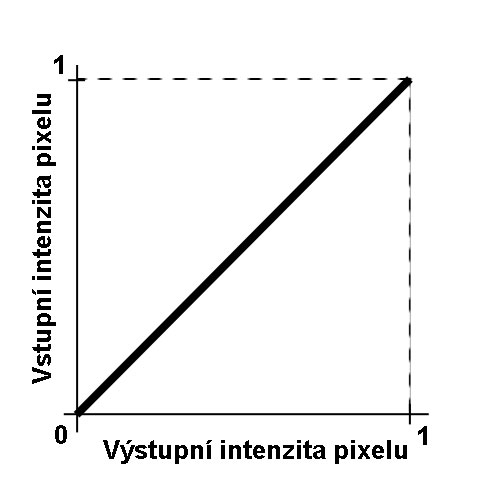
\includegraphics[width=0.7\textwidth,height=0.7\textwidth]{Text/IMG/Kontrast_Identita.jpg}
\end{center}
%\caption{Křivka znázorňující barevnou transformaci, při které se snímek nezmění.}
%\label{kontrastKrivka}
%\end{figure}

Pixel o vstupní intenzitě $0.25$ bude mít výstupní intenzitu $0.25$.

Ukažme si nyní, jak vypadá stejná křivka pro transformaci, která kontrast obrázku zvyšuje, např. pro $ c_{contrast}=1.25 $.
Vezmeme-li v úvahu uvedený vzorec a vezmeme-li dále v úvahu podmínku $ Im(x,y) \in [0,1] $.

Pak můžeme křivku transformace pro $ c_{contrast}=1.25 $ načrtnout takto:


%\begin{figure}
\begin{center}
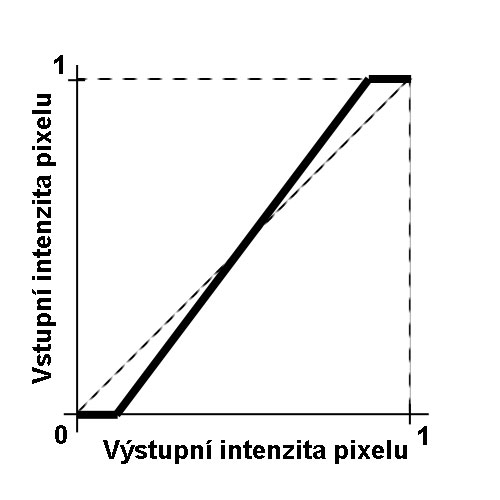
\includegraphics[width=0.7\textwidth,height=0.7\textwidth]{Text/IMG/Kontrast_Transformace_1.jpg}
\end{center}
%\caption{Transformační křivka změny kontrastu.}
%\label{kontrastKrivka}
%\end{figure}

Křivka na obrázku má strmější spád. To znamená, že světlejší pixely (s původní světlostí $> 0.5$) se staly ještě světlejší a naopak tmavší pixely (s původní světlostí $< 0.5$) ještě více ztmavly. Z uvedeného nákresu je pak vidět co vyplývá z předpisu transformace a podmínek $ Im(x,y) \in [0,1]$. Při zvýšení kontrastu koeficientem k se intenzita všech bodů, jejichž intenzita je z intervalu $ [0,\frac{1}{2k}] $, změní na $0$ a dále intenzita všech bodů, jejíchž původní intenzita byla v intervalu $[1-\frac{1}{2k},1]$, se změní na hodnotu $1$. Jinými slovy, jak se v odborné terminologii užívá, dojde ke ztrátě grafické informace a to v uvedených množinách bodů. Volnější parafrázi bychom řekli, že odstíny největlejší bodů se slijí do jediného odstínu a odstíny nejtmavších bodů se slijí do jediného odstínu (viz tabulka \ref{highcontrast}).

\begin{table}%[ht]
	\caption{Příklad příliš výrazné změny kontrastu, kdy dochází ke ztrátě grafické informace.}
\label{highcontrast}
		\begin{tabular}{p{7cm}p{7cm}}
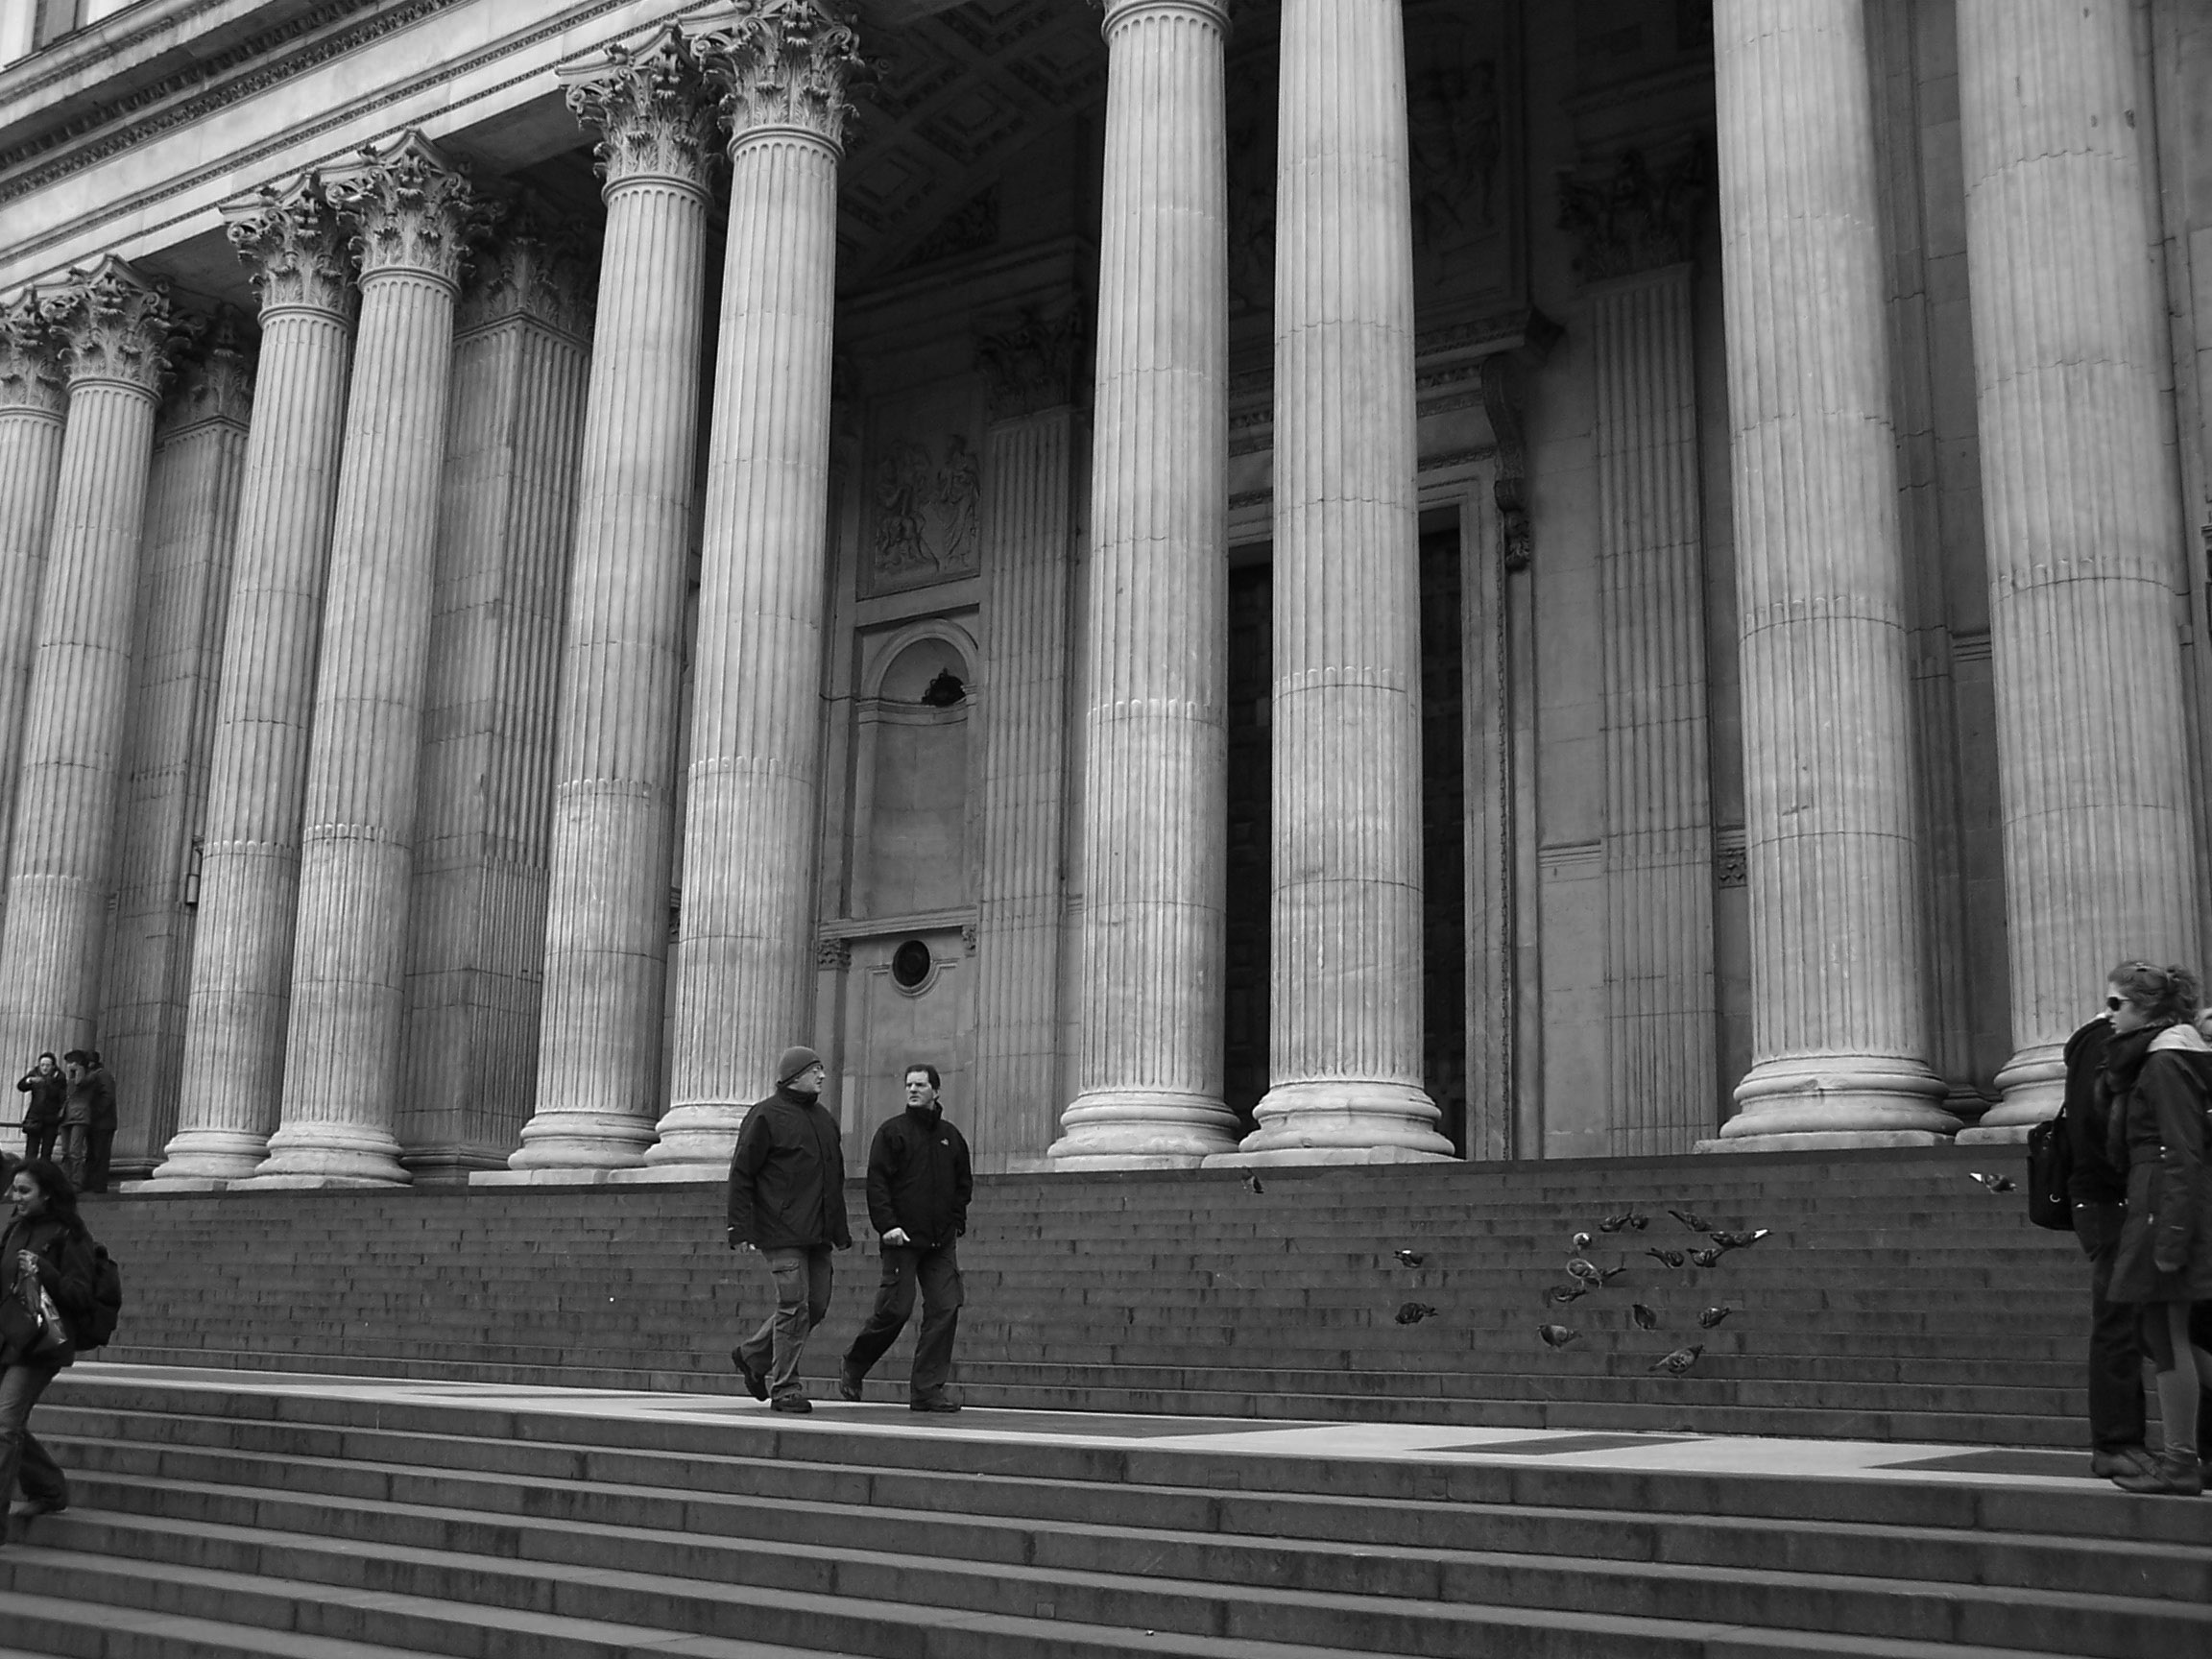
\includegraphics[width=0.5\textwidth,height=0.35\textwidth]{Text/IMG/London.jpg} & 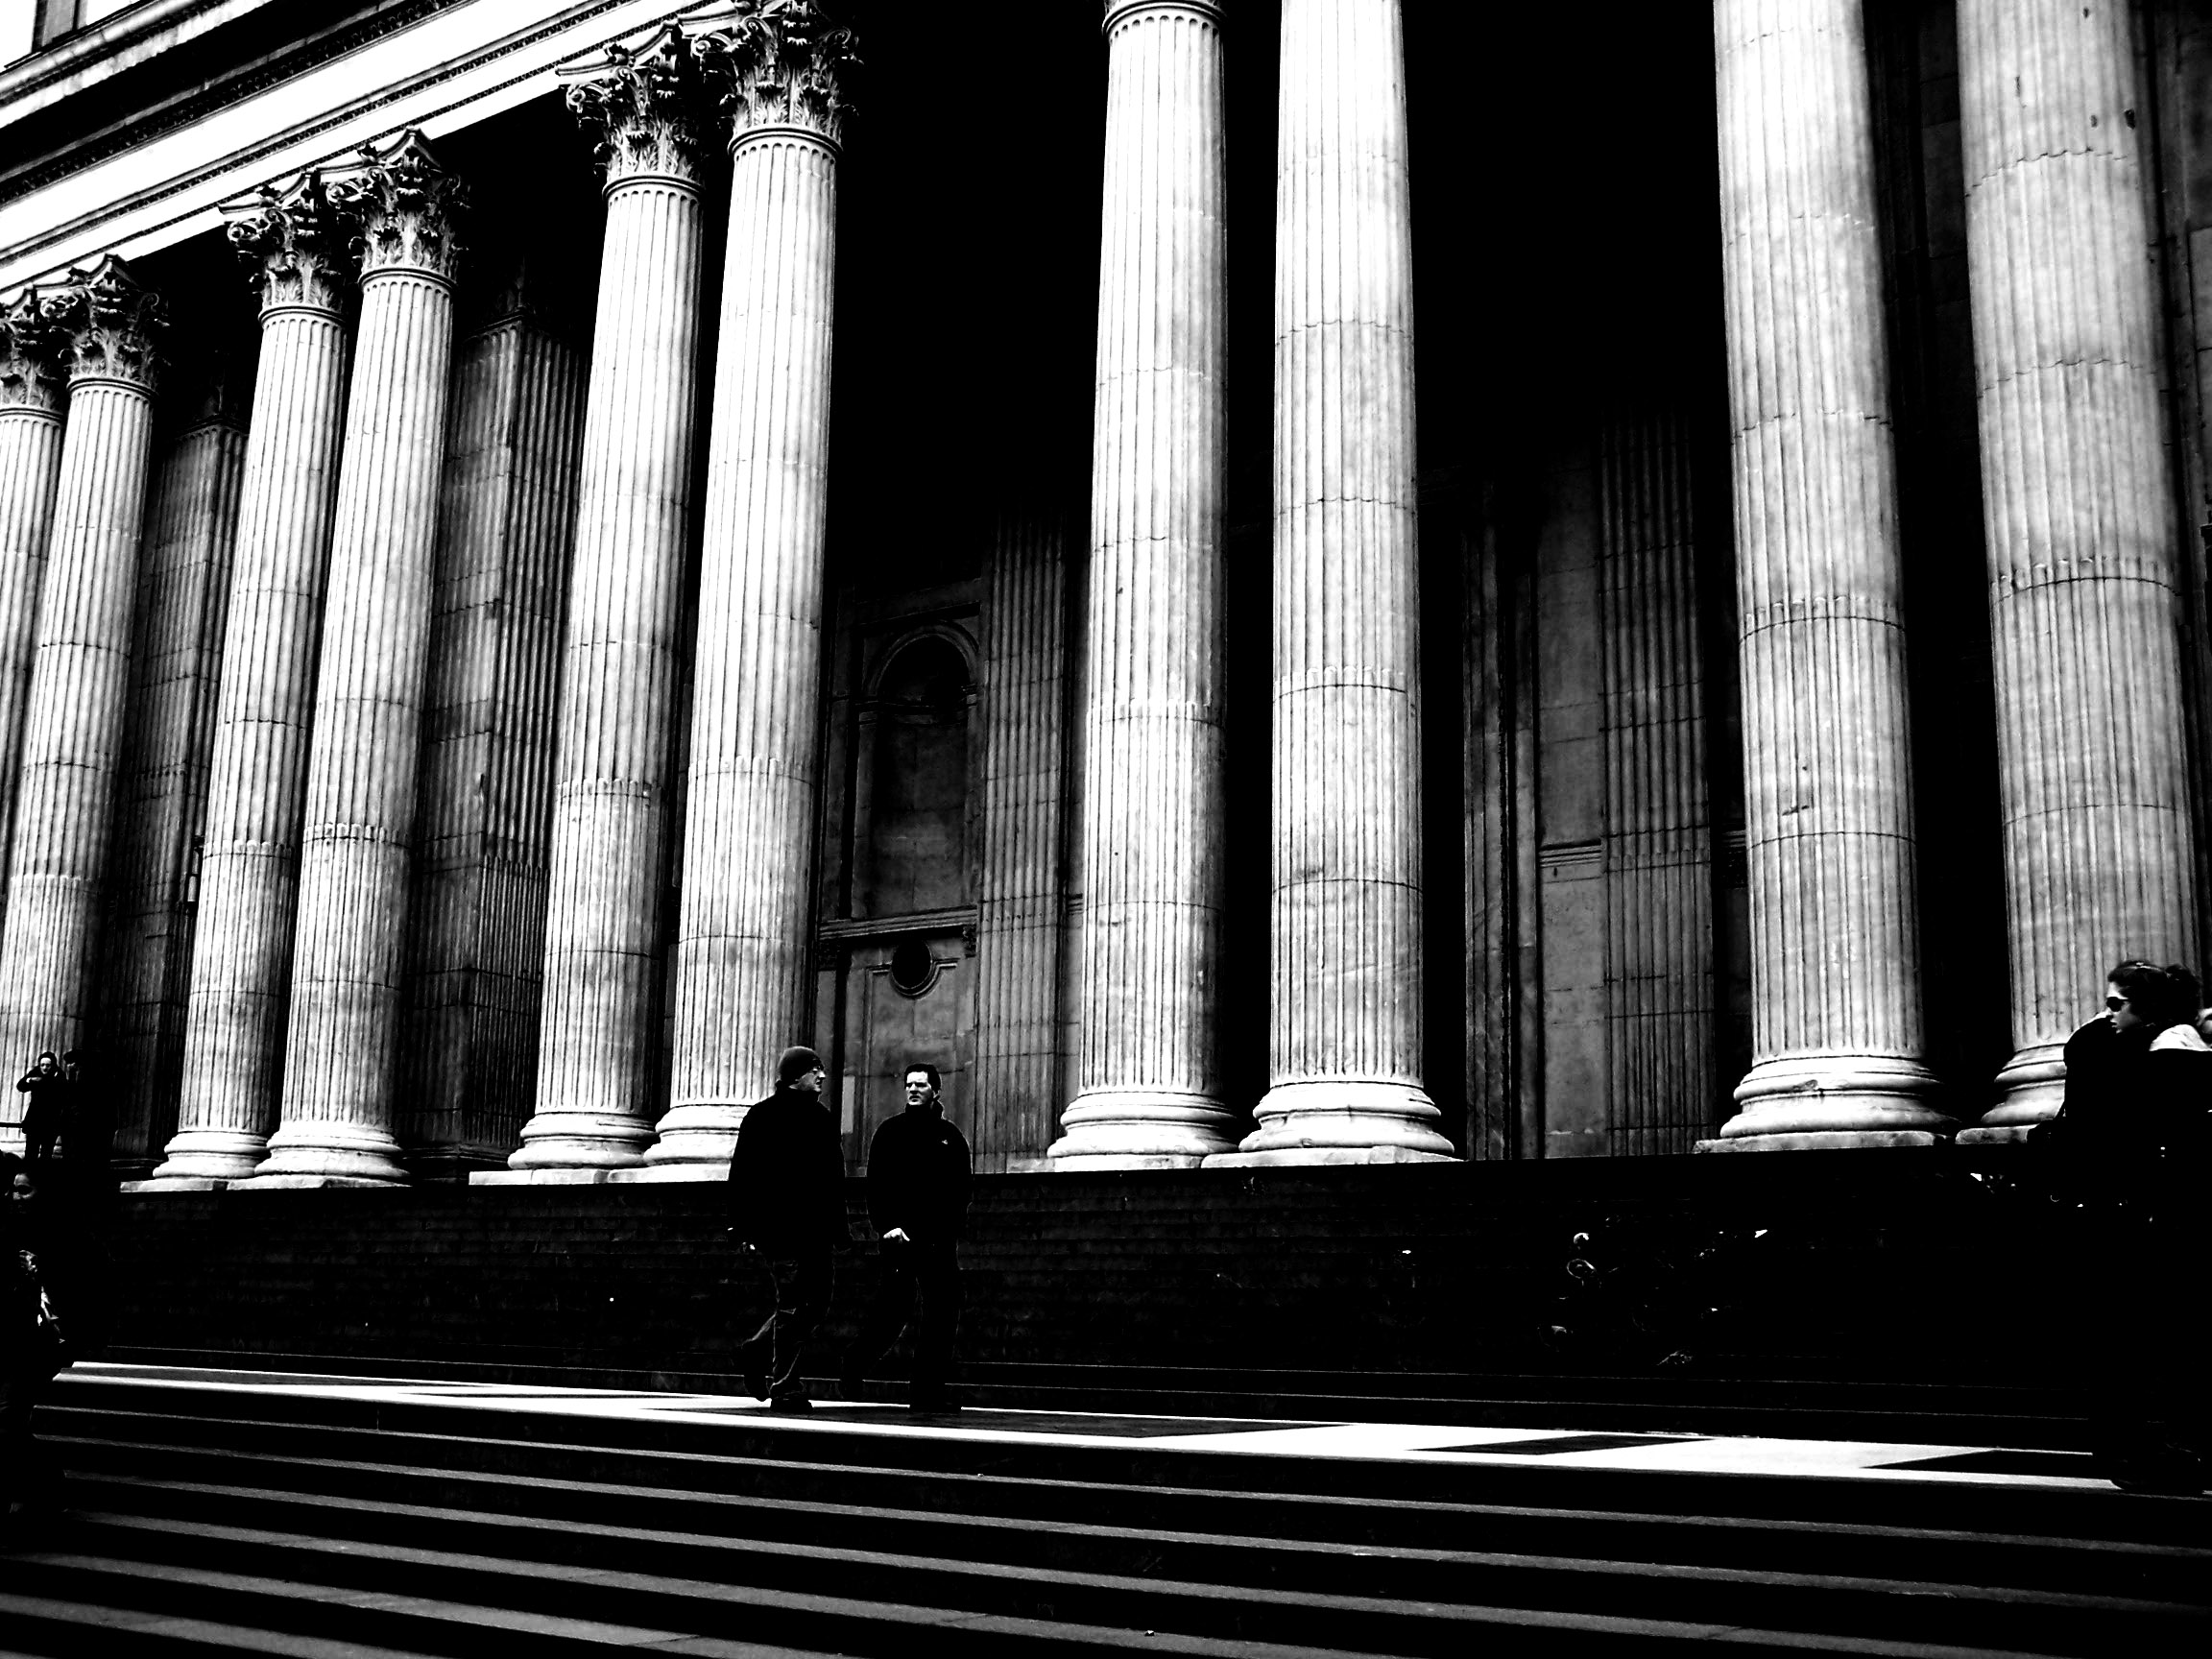
\includegraphics[width=0.5\textwidth,height=0.35\textwidth]{Text/IMG/London_High_Contrast.jpg} \\
\center{Původní obrázek.} & \center{Obrázek po změně kontrastu.}\\
		\end{tabular}
\end{table}

Nejmodernější počítačové programy pak používají nelineární transformace pro změnu kontrastu. Při jejich použití nedochází ke ztrátě grafické informace. Křivka takové transformace pak vypadá přibližně takto: 

\begin{center}
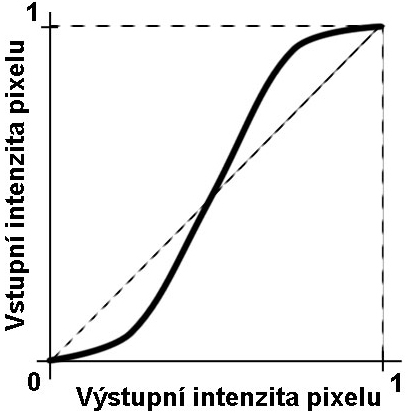
\includegraphics[width=0.7\textwidth,height=0.7\textwidth]{Text/IMG/Kontrast_Transformace_2.jpg}
\end{center}

\subsection{Kontrast v OpenGL}
Knihovna OpenGL nenabízí funkce pro změnu kontrastu snímku. Knihovna nabízí pouze funkce manipulující s parametry: bias, scale.

Parametr bias je koeficient, kterým násobíme barevnou složku pixelu. Podíváme li se znovu na graf zobrazující křivku barevné transformace, pak pro bias=1,5 bude křivka vypadat takto:

\begin{center}
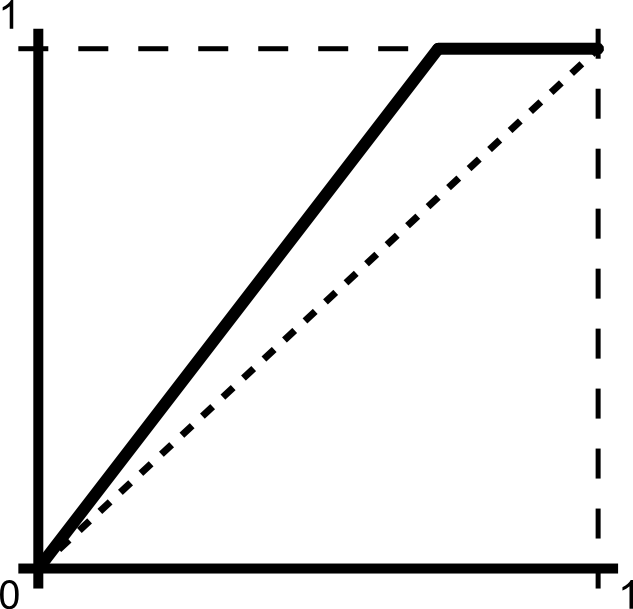
\includegraphics[width=0.5\textwidth]{Text/IMG/Bias.png}
\end{center}

Parametrem bias tedy násobíme barvu každého pixelu (hodnota je pak automaticky oříznuta na přípustnou mez). Lze to interpretovat tak, že parametr bias mění směrnici transformační křivky.

Chceme-li provést změnu kontrastu snímku, nestačí nám pouze násobit barvu všech pixelů a změnit tak sklon transformační křivky. Musíme dále křivku posunout aby neprocházela bodem (0,0), ale (0.5,0.5), jak je vidět na obrázku \ref{kontrastKrivka}.

Parametr scale dokáže přičíst konstantu k barevné hodnotě všech pixelů. Znamená to tedy, že parametr scale mění jas snímku. Viz graf:

\begin{center}
\includegraphics[width=0.5\textwidth]{Text/IMG/Scale.png}
\end{center}

Jak lze předpokládat z obou příkladů, zkombinujeme-li obě transformace, tj. změníme-li směrnici transformační křivky grafu a posuneme-li ji o správnou hodnotu, lze dosáhnout transformace, která odpovídá změně kontrastu.

Volme parametry:

Bias = 1.2
Scale = -0.1

Pak graf bude vypadat:

\begin{center}
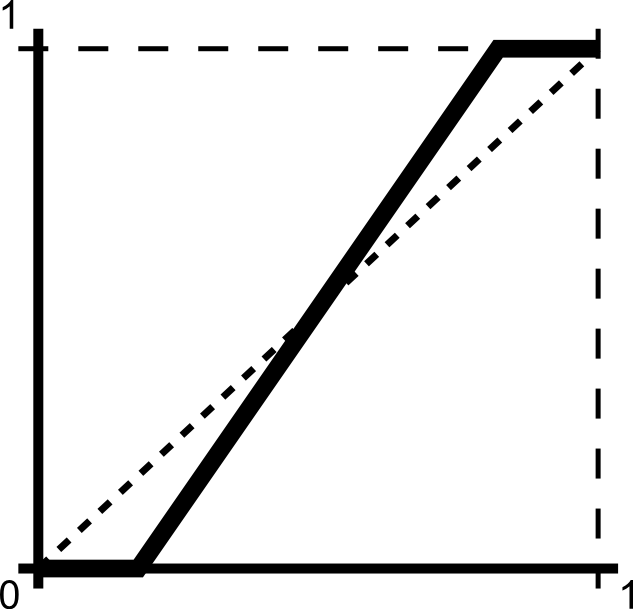
\includegraphics[width=0.5\textwidth]{Text/IMG/BiasScale.png}
\end{center}

Jak plyne z předchozího, pomocí parametrů Bias a Scale lze docílit změny kontrastu snímku. Pomocí parametru Scale lze docílit změny světlosti.

\subsection{Kontrast v knihovně Cg}
Knihovna Cg toolkit nám nabízí programování vlastních výpočtů s barvou pixelů. Paleta možných transformací je pak velice široká a implementace je jednoduchá - program napíšeme v jazyku Cg, který je velice podobný jazyku C.

Implementace změny kontrastu pak bude vypadat:
\begin{lstlisting}[label=DicomImageClass,caption={...}]
C3E3f_Output main(float2 texCoord : TEXCOORD0, uniform sampler2D decal : TEX0, uniform float brightness){
  C3E3f_Output OUT;
  OUT.color = tex2D(decal,texCoord)*bias - scale;
  return OUT;
}
\end{lstlisting}

Ve srovnání s OpenGL je tato implementace výrazně přehlednější. Podíváme-li se na řádek 3, vidíme hned zápis transformační funkce ve tvaru: f(x) = k*x - z. Jak již lze předpokládat: s jazykem Cg můžeme jednoduše popisovat mnohem složitější transformace využívající elementárních matematických funkcí: log, exp, sin.




\subsection{Závěr}
Z programu DicomPresenter je možné odstranit knihovnu Cg. Omezíme-li se v programu na použití pouze elementárních obrazových transformací: kontrast a jas, můžeme tyto implementovat i v OpenGL. Důvodem, proč je v programu použita knihovna Cg toolkit, bylo v práci \cite{neskudla} uvedeno, že bez ní dojde při vícenásobné transformaci oříznutí barev obrázku: když kontrast hodně zvýšíme a opět snížíme, vytrarí se z obrázku část původní informace. Toto však lze obejít, uložíme-li si snímek do paměti dvakrát: původní s nezměněným kontrastem a výsledný po změně, který zobrazíme uživateli. Bude-li si přát uživatel další změnu kontrastu, nebudeme jí počítat ze snímku, který vidí, ale z původního, jež je uložen v paměti. Nevýhoda tohoto řešení je ta, že pro dvojrozměrné snímky budeme zatěžovat operační paměť dvojnásobkem dat. Vzhledem k tomu, že snímky jsou uloženy v paměti grafické karty je toto omězení poměrně vážné (pro starší grafické karty).



\newpage
\section{Rychlost vykreslování}
Jednou z otázek, na kterou se snaží najít odpověď tento VÚ je to, zda by bylo možné odstranit z programu knihovny Cg, OpenGL. Bylo tedy potřeba zjistit, jaký dopad by mělo odstranění knihoven OpenGL, Cg na funkčnost programu. Jedná se o knihovny usnadňující vykreslování obrazových dat. Zároveň se ale jedná o knihovny urychlující vykreslování dat. Při odstranění knihoven by se tak mohlo stát, že program nebude schopen dostatečně rychle vizualizovat data a nebude tak možné v reálném čase vykreslovat to, co uživatel dělá.

Pro zjištění toho, jaký dopad bude mít absence knihoven na výkon, bylo potřeba nějakým způsobem změřit rychlost renderování s využitím grafických knihoven a bez nich. K tomuto účelu byly zkonstruovány tři testovací programy, každý z nich obohacen o podporu nějaké specifické grafické knihovny. První program využíval jen grafickou podporu v knihovně Qt, druhý využíval podpory Qt a OpenGL, třetí pak všech tří knihoven: Qt, OpenGL, Cg toolkit. Jako cíl programů bylo stanoveno změnit světlost snímku a vykreslit jej na obrazovku. Aby bylo možné naměřit relevantní data, necháme operaci běžet v cyklech několikrát za sebou.

Pro zjištění toho, jaký dopad na funkčnost programu bude mít absence knihovny OpenGL, respektive Cg, byly nejprve zkonstruovány tři testovací programy. Všechny tři programy měli za cíl co nejvíckrát za sebou vykreslit stejný snímek, v každém kroku ale provedli se snímkem jednoduchou barevnou úpravu. Programy se lišili v tom, které z knihoven využívali. První se opíral jen o grafické funkce Qt knihovny, druhý využíval k vizualizaci Qt i OpenGL, třetí pak Qt, OpenGL i Cg toolkit. Smyslem bylo porovnat rychlost vykreslování všech tří variant. Jako testovací grafickou operaci jsme si vybrali jednoduché násobení všech barevných složek každého pixelu konstantou.

Výsledky testování vypovídaly o značném zpomalení při nepřítomnosti knihovny OpenGL v programu. Z toho se daly vyvozovat závěry, že knihovnu OpenGL nebude možné z programu odstranit (viz závěr této kapitoly - řádové zpomalení). Nicméně po konzultaci se školitelem, se podařilo objevit implementaci stejné úlohy pouze v knihovně OpenGL, která však byla téměř o řád rychlejší. Vzhledem k tomu, že pomalejší implementace je intuitivnější, zatímco rychlejší tak intuitivní neni, ale využívá hlubších poznatků problematiky datové reprezentace ukládání snímků, uvádíme obě implementace.

\begin{tabular}{| l | l | }
  \hline                       
  Varianta 1 & Qt\\
  \hline
  Varianta 2 & Qt, OpenGL\\
  \hline
  Varianta 3 & Qt, OpenGL, Cg toolkit \\
  \hline  
\end{tabular}

\subsection{Implementace v Qt}
Grafická část rozhraní knihovny Qt je dělaná čistě pro dvojrozměrnou grafiku a všechny výpočty jsou prováděny jen na procesoru. Chceme-li měnit světlost snímku, musíme procházet for-cyklem všechny body obrázku a provést operaci pro každý bod zvlášť. Pokud navíc zadáme světlost pixelu mimo požadovanou mez, program se zasekne. Narozdíl od toho knihovny OpenGL i Cg automaticky barevnou hodnotu pixelu oříznou na přípustnou mez.

Intuitivní, avšak pomalejší implementace v Qt knihovně vypadá následovně:

\begin{lstlisting}[label=DicomImageClass,caption={...}]
	start = time (NULL);
	QLabel label;
	QImage MemoryImage("D:/Workspace/Qt/Picture.png");
	QImage ShowImage("D:/Workspace/Qt/Picture.png");
	label.setPixmap(QPixmap::fromImage(ShowImage));
	label.show();
	qreal H, S, V;
	QColor Color;
	qreal contrast=0;
	for (int j=0; j<10; j++){
		cont = 0;
		for (int i=0; i<99; i++){
			cont=cont+0.01;
			ShowImage = MemoryImage;
			for ( int y = 0; y < h; y++ ){
				for ( int x = 0; x < w; x++ ){
					Rgb = MemoryImage.pixel(x,y);
					Rgb = qRgb(qRed(Rgb)*cont,qGreen(Rgb)*cont,qBlue(Rgb)*cont);
					ShowImage.setPixel(x,y,Rgb);
				}
			}
			label.setPixmap(QPixmap::fromImage(ShowImage));
			label.repaint();
		}
	}
	end = time (NULL);
\end{lstlisting}

V úryvku kódu vidíme zejména procházení celého obrázku ve dvou for-cyklech(řádky 13,14). V každém kroku si zjistíme barevné souřadnice pixelu, upravíme je a uložíme je. To má na starosti procesor a jedná se o největší handicap celého programu. Při této implementaci je úloha zpracována sériově na jednom jádře, jak je vidět z následujících grafů sledujících zátěž jednotlivých jader:

\hspace{1cm}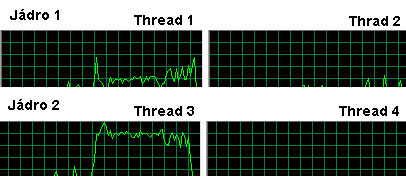
\includegraphics[width=0.8\textwidth]{Text/IMG/MultiThread.jpg}

Procesor je fyzicky dvoujádrový, ale operační systém jej vidí jako čyřjádrový. Celý výpočet probíhal viditelně v třetím threadu, v prvním pak běžely zřejmě jen pomocné operace, další 2 thready zůstaly nevyužité.

Chceme-li výpočet urychlit, můžeme tak udělat v několika krocích:

Nebudeme si ukládat barevné souřadnice původního obrázku do proměnné, tam je upravovat a ukládat zpět na půbodní místo. Ale necháme si předat ukazatel na místo v paměti, kde je obrázek uložen, a výsledek ukládat přímo tam.

Dále nebudeme volat funkci, která nám na základě souřadnic vrátí barevné složky obrázku, ale necháme si od Qt knihovny předat ukazatel na celý jeden řádek obrázku. Tím se vyhneme opakovanému volání funkce.

Dvojice for-cyklů procházející obrázek bude nahrazena tímto kódem:

\begin{lstlisting}[label=DicomImageClass,caption={...}]
for (int i=0; i<99; i++){
	cont=cont+0.01;
	ShowImage = MemoryImage;
	for ( int y = 0; y < h; y++ ){
		Rgb = (QRgb*)ShowImage.scanLine(y);
		for ( int x = 0; x < w; x++ ){
			Rgb[x] = qRgb(qRed(Rgb[x])*cont,qGreen(Rgb[x])*cont,qBlue(Rgb[x])*cont);
		}
	}
	label.setPixmap(QPixmap::fromImage(ShowImage));
	label.repaint();
}
\end{lstlisting}

Jak je vidět, v každém řádku obrázku ušetříme hned dvě volání funkce pro každý pixel. Zkusme si spočítat kolik funkčních volání jsme ušetřili:

V prvním případě voláme pro každý pixel funkce QImage::pixel() a QImage::setPixel(). Rozměr obrázku je 512*512 pixelů. To jest: 512*512*2 = cca 500 000 funkčních volání.

V druhém případě voláme pouze funkci QImage::scanLine pro každý řádek obrázku, tj. 512*2 = 1024 volání.

Jak je vidět, jedná se o zredukování počtu volání nějaké funkce o dva řády. Výsledek takového zjednodušení uvidíme v závěru kapitoly.


\subsection{Implementace v OpenGL}

OpenGL je knihovna přímo určená pro urychlení grafických výpočtů a jejich zjednodušenou obsluhu. Hlavní rozdíl oproti implementaci v Qt je ten, že výpočty neprobíhají na procesoru, ale na grafické kartě, což je, jak se později ukáže, zásadní rozdíl ve výkonnosti programu. Stejně tak data nejsou uložena v modulech paměti RAM na základní desce, ale jsou v paměti grafické karty.

Implementace vypadá následovně:

\begin{lstlisting}[label=DicomImageClass,caption={...}]
start = time (NULL);
for (int j=0; j<10; j++){
	float Brightness=0.0;
	for (int i=0; i<1000; i++){
		Brightness = Brightness+0.001;
		gl->Paint(Brightness);
		w.updateGL();
	}
}
end = time (NULL);

void GLPainter::PrepareTexture() {
	glBindTexture( GL_TEXTURE_2D, TextureIdentifier );
	gluBuild2DMipmaps( GL_TEXTURE_2D, 3, width, height, GL_RGB, GL_UNSIGNED_BYTE, TextureData );
	glEnable( GL_TEXTURE_2D );
}

void GLPainter::Paint(float Brightness){
	glBegin(GL_POLYGON);
		glColor3f (Brightness, Brightness, Brightness);
		glTexCoord3f(0.0,0.0,0.0);	glVertex3f( -1.0, -1.0, 0.0 );
		glTexCoord3f(0.0,1.0,0.0);	glVertex3f( -1.0,  1.0, 0.0 );
		glTexCoord3f(1.0,1.0,0.0);	glVertex3f(  1.0,  1.0, 0.0 );
		glTexCoord3f(1.0,0.0,0.0);	glVertex3f(  1.0, -1.0, 0.0 );
	glEnd();
}
\end{lstlisting}
Na první pohled lze vidět nesrovnatelné zjednodušení kódu, zatímco v prvním případě (Qt) jsme museli procházet celý obrázek po pixelech, zde můžeme využít funkce knihovny OpenGL pomocí které lze měnit světlost jejího výstupu.

V programu si nejprve snímek uložíme do paměti jakožto OpenGL texturu (řádky 12-16), posléze provádíme vykreslování této textury na načrtnutý obdélník (18-26).


\subsection{Iplementace v Cg}

Knihovna Cg slouží k programování výpočtů na čipu grafické karty. V jednoduchém jazyku podobném jazyku C popíšeme prováděné výpočty pro změnu světlosti. Výpočty jsou pak realizovány na speciálním hardwarovém čipu (pixel shader, vertex shader). Přínos pixel a vertex shaderů je v nové paletě efektů, jež je možno provádět, a dále ve výrazném urychlení těchto efektů.

Podívejme se na implementaci programu s využitím Cg, tentokráte výpočty nebyly prováděny jen v prostředí jazyka C++, ale i v jazyce Cg.

\begin{lstlisting}[label=DicomImageClass,caption={...}]
start = time (NULL);
for (int j=0; j<10; j++){
	float Brightness=0.0;
	for (int i=0; i<1000; i++){
		Brightness = Brightness+0.001;
		gl->Paint(Brightness);
		w.updateGL();
	}
}
end = time (NULL);

void GLPainter::PrepareTexture() {
	glBindTexture( GL_TEXTURE_2D, TextureIdentifier );
	gluBuild2DMipmaps( GL_TEXTURE_2D, 3, width, height, GL_RGB, GL_UNSIGNED_BYTE, TextureData );
	glEnable( GL_TEXTURE_2D );
}

void GLPainter::changeBrightness( float Brightness ){
	cgGLBindProgram(Program);
	cgGLEnableProfile(Profile);
	cgSetParameter1f(hBright, Brightness);
	cgUpdateProgramParameters (Program);
	cgGLDisableProfile(Profile);

	Paint();
}

void GLPainter::Paint(){
	glClear(GL_COLOR_BUFFER_BIT);

	cgGLBindProgram(Program);
	cgGLEnableProfile(Profile);
	cgGLEnableTextureParameter(hDecal);

	glBegin(GL_POLYGON);
		glTexCoord3f(0.0,0.0,0.0);	glVertex3f(-1.0,-1.0,0.0);
		glTexCoord3f(0.0,1.0,0.0);	glVertex3f(-1.0,1.0,0.0);
		glTexCoord3f(1.0,1.0,0.0);	glVertex3f(1.0,1.0,0.0);
		glTexCoord3f(1.0,0.0,0.0);	glVertex3f(1.0,-1.0,0.0);
	glEnd();

	cgGLDisableProfile(Profile);
	cgGLDisableTextureParameter(hDecal);
}
\end{lstlisting}

\begin{lstlisting}[label=DicomImageClass,caption={...}]
struct C3E3f_Output {
  float4 color : COLOR;
};

C3E3f_Output main(float2 texCoord : TEXCOORD0, uniform sampler2D decal : TEX0, uniform float brightness)
{
  C3E3f_Output OUT;
  OUT.color = tex2D(decal,texCoord)*brightness;

  return OUT;
}
\end{lstlisting}

První část programu je shodná s předchozí verzí (opět je volána knihovna OpenGL). Rozdíl však začíná od řádku 18. Ve funkci changeBrightness() musíme volat funkce knihovny Cg toolkit pomocí kterých předáme pixel shaderu parametr určující změnu světlosti. Před samotným vykreslováním pomocí OpenGL (řádky 35-40) musíme nechat program zkompilovat na čipu grafické karty a nastavit, aby ovlivňoval výstup OpenGL.

Za povšimnutí stojí fakt, že výpočet změny světlosti se přesunul z kódu C++ do Cg. Změna světlosti je popsána v samostatném programu jež se kompiluje na grafické kartě.


\subsection{Porovnání výpočtů}

Popsané programy byly testovány na počítačové sestavě:

Intel Core i3, ATI Radeon 5470. Takt procesoru je 2,26 GHz

Jedná se o dvoujádrový procesor, pro výpočet však bylo použito pouze jedno jádro. Takt GPU na grafické kartě je 750MHz.

V každé konfiguraci jsme požadovali jiný počet cyklů programu, jenom z důvodu časové úspory při ladění.

\begin{tabular}{| p{5cm} | l | l | l | }
  \hline                       
  Typ konfigurace & Počet cyklů & Čas & Snímků za vteřinu \\
  \hline
  \hline
  Qt (bez přímého přístupu do paměti)& 100 & 4 sekundy & 25 fps\\
  \hline
  Qt (s přímým přístupem do paměti)& 1000 & 11 sekund & 90 fps\\
  \hline
  Qt, OpenGL & 10 000 & 16 sekund & cca 600  fps \\
  \hline
  Qt, OpenGL, Cg & 10 000 & 14 sekund & cca 700 fps \\
  \hline  
\end{tabular}

Jak je vidět z namšřených údajů, s použitím knihovny OpenGL se dá dosáhnout úctihodného výkonu při vykreslování snímků v programu. Nicméně vezmeme-li v úvahu fakt, že standardní rychlost snímání ovládacích zařízení přes USB v operačním systému je 125Hz a dále obnovovací frekvence u monitoru nebývá zpravidla vyšší než 100Hz, musíme uznat, že výkon dosažený pomocí OpenGL je nadbytečný. To by určitě nevadilo a velká rezerva ve výkonu by mohla být zárukou plynulého chodu programu i za ztížených podmínek (uživatel využívá procesor i jiným způsobem za běhu programu), ale bohužel přítomnost knihovny OpenGL v programu má za důsledek značné problémy s provozem programu na méně výkonných, či starších grafických kartách. Byly zjištěny problémy s provozem programu na integrovaných grafických kartách Intel, které však jsou velice často instalovány do moderních notebooků.

Výkon programu, při pomalejší implementaci v Qt knihovně, kdy jsme nevyužívali manuálního přístupu do paměti, ale k tomuto jsme používali implementované funkce v Qt knohovně, je spíše nedostačující. Dosažený výkon v testovacím programu: 25 snímků za vteřinu sice sám o sobě dostačující je, ale musíme vzít v úvahu ten fakt, že se jednalo o velice primitivní testovací program, který nedělal nic jiného než přepočet barevných složek obrázku a jeho zobrazení. DicomPresenter vedle toho musí vykreslovat ovládací prvky programu, což znamená několik funkčních volání navíc.

Oproti tomu výkon dosažený pomocí pokročilé implementace, kdy přistupujeme ručně do paměti počítače a obrazová data měníme tam, by měl být dostačující pro běh reálného programu. I při výrazném zpomalení aplikace kvůli přepočítávání zobrazovaných ovládacích prvků, bychom se měli bezpečně udržet nad hranicí 30FPS.

Závěrem této kapitoly je nutno podotknout, že Knihovny OpenGL, Cg z programu odstranit lze a v nejbližší době bude takto učiněno. Program by se tak měl stát výrazně bezproblémovější, co se týče provozu v praxi. Měl by být kompatibilní s převážnou většinou počítačových sestav - to je však nutná podmínka pro to, aby program mohl být v praxi použitelný.






\newpage
\section{Konfigurace pro překlad}
\label{sec:preklad}
Program Dicom-Presenter je závislý na více než pěti externích knihovnách. Překlad programu se tak stává mírně komplikovaný. Při překladu programu je potřeba obstarat přeložené verze všech knihoven. Knihovny Qt, OpenGL, Cg jsou od výrobce vždy k dispozici pro různé typy OS včetně OS Windows. Situace se zbylými knihovnami je výrazně horší. Knihovny dcmtk a plib je vždy nutné nejprve zkompilovat. Při překladu je pak nutné si vybrat způsob přeložení podle následujících možností: Single-Thread nebo Multi-Thread, Static linking nebo Dynamic linking, realease nebo debug. Konfigurace překladu by měla být pro všechny dílčí knihovny i pro samotnou aplikaci totožná. To může být problém, neboť například výrobce knihovny dcmtk dokládá, že není vhodné jí přeložit jako dynamickou .dll. Výrobce Qt knihovny zas svou knohovnu dodává pouze jako .dll. Tím vznikají značné komplikace. Tato kapitola popíše základní problematiku konfigurací překladu.

\subsection{Microsoft Visual C++ Runtime}
Důvodem, proč všechny součásti programu musí být přeloženy ve stejné konfiguraci je to, že při překladu v prostředí Visual Studio je při každé dílčí konfiguraci k programu přiložena specifická verze knihovny C++ Runtime.

V knihovně C++ Runtime jsou obsaženy základní funkce C++. Při překladu je C++ Runtime vždy linkována k aplikaci. Programátorovi tedy stačí vždy jen odkázat na požadovaný hlavičkový soubor s potřebnou funkcí, např. \clist{\#include <stdio.h>}.

Zmiňme jen orientačně jaké součásti můžeme v C++ Runtime nalézt:

\hspace{-0.5cm}
\begin{tabular}{| p {2cm}| l | p{6cm}| }
  \hline                       
  Název hlavičkového souboru & Příklad funkcí & Popis funkcí \\
  \hline
  \hline
  stdio.h & printf, getchar, fwrite, fread & Práce s vstupem a výstupem aplikace (standartní I/O i soubory). \\
  \hline  
  stdlib.h & malloc, free, atof, div & Práce s pamětí (alokace paměti, uvolnění paměti), přetypování proměnných aj.  \\
  \hline  
  math.h & sin, cos, exp & Knihovna s elementárními matematickými funkcemi.  \\
  \hline  
  time.h & tm\_sec, tm\_hour & Knihovna pro získání informací o aktuálním čase, všechny funkce vrací typ int.  \\
  \hline  
\end{tabular}

Při překladu je tedy nutné hledět na to, aby ke všem součástem byla přiložena stejná verze C++ Runtime knihovny a nekřížit např. MSVCRT.lib s LIBC.lib (viz konec této kapitoly).

\subsection{Konfigurace překladu}
Program, respektive jeho součásti je možné překládat celkově v těchto šesti různých konfiguracích:

\hspace{-0.5cm}
\begin{tabular}{| l|| p{5cm} | p{5.5cm}  |}
  \hline                       
  Release & Single-Thread & Multi-Thread \\
  \hline
  \hline                     
  Static Link & Single-Thread, Static Link, Release & Multi-Thread, Static Link, Release\\
  \hline
  Dynamic Link & --- & Multi-Thread, Dynamic Link, Release\\
  \hline  
\end{tabular}

\hspace{-0.5cm}
\begin{tabular}{| l|| p{5cm} | p{5.5cm}  |}
  \hline                       
  Debug & Single-Thread & Multi-Thread \\
  \hline
  \hline                     
  Static Link & Single-Thread, Static Link, Debug & Multi-Thread, Static Link, Debug\\
  \hline
  Dynamic Link & --- & Multi-Thread, Dynamic Link, Debug\\
  \hline  
\end{tabular}

Pro každou verzi překladu linkujeme jinou verzi C++ Runtime knihovny.
Proberme si nyní rozdíly mezi konfiguracemi:

\subsection{Statické vs. dynamické knihovny}
Při překladu dílčí části kódu si musíme vybrat, zda kód chceme kompilovat do statické nebo dynamické knihovny. Statické knihovny zpravidla končí příponou .lib (windows), případně .a (linux). Dynamické knihovny mají na Windows známou příponu .dll, na Unixových OS mají pak příponu .so (shared object). Bohužel, často je u OS Windows potřeba mít správnou verzi .dll knihovny. Verzi knihovny někdy lze vyčíst z názvu knihovny: např. \clist{msvcrt70.dll} a \clist{msvcrt71.dll}. V případě Unixových operačních systémů je situace značně přehlednější: verze knihovny se zpravidla píše na konec názvu souboru: např. \clist{libQtCore.so.4}, \clist{libQtCore.so.3}. Symbolickým linkem je pak vytvořen zástupce \clist{libQtCore.so}, který zpravidla ukazuje na nejnovější verzi knihovny. Pokud však nějaká aplikace potřebuje starši verzi knihovny, automaticky hledá název \clist{libQtCore.so.3}. Při instalaci novější verze knihovny: např. \clist{libQtCore.so.4.1} se pak změní symbolický link na nejnovější verzi, ale všechny starší verze mohou zůstat v programu zachovány. Systém knihoven je tak výrazně přehlednější.

DLL knihovny jsou zpravidla umístěny v adresáři \clist{Windows/system32}, dále bývají ponechány v adresáři programu, který je používá. Na Unixových OS jsou sdílené knihovny (\clist{.so}) umístěny v adresáři \clist{/usr/lib}. Zde je opět patrný značný rozdíl v systematičnosti obou operačních systémů. Zatímco na OS Windows jsou \clist{.dll} soubory umístěny v adresáři \clist{/system32}, na Unixových OS jsou \clist{.so} soubory přehledně rozděleny do podadresářů. Všechny \clist{.so} soubory knihovny Qt knihovny tak nalezneme v adresáři: \clist{/usr/lib/qt4}.

\subsection{Single-thread vs. Multi-thread}
Při překladu je dále třeba si vybrat, zda má být aplikace přeložena s podporou více vláken. Připojení runtime knihovny s vícevláknovou podporou pak umožní používání příkazů k práci s vlákny.

Vícevláknové programování se používá zejména u aplikací s grafickým rozhraním, kde je potřeba provést nějakou časově náročnější operaci, vedle toho je ale potřeba neostále obsluhovat grafické rozhraní. Dobrým příkladem je emailový klient: po stisknutí tlačítka odeslat začne odesílání emailu, tj. komunikace se serverem, přenášení dat atd. Během těchto akcí by uživatel u jednovláknové aplikace musel čekat, až vše doběhne do konce, rozdělíme-li odesílání mailu a chod GUI do dvou nezávislých vláken, může uživatel manipulovat s programem i během odesílání emailu.

Bohužel používání více vláken je věc úzce spjatá s operačním systémem, pro OS Windows se používají funkce z hlavičkového souboru windows.h. Proto musíme při psaní aplikace, jejíž kód má být přenositelný mezi více operačními systémy použít nějakou knihovnu, která práci s vlákny obstará. Příkladem může být knihovna OpenMP. Práce s vlákny v OpenMP se pak obstarává použitím maker překladače. Další knihovnou, jež je portována pro OS Linux i Windows, je knihovna pthreads. Práce s vlákny v pthreads již bohužel není natolik zjednodušena jako v případě OpenMP. V pthreads musíme ručně vytvářet jednotlivá vlákna.

\subsection{Realase vs. Debug}
\label{releasedebug}
Další z možností výběru je Debug vs. Release. Překlad se liší v tom, že při debug překladu jsou do kódu vloženy dodatečné informace, které slouží k ladění programu. Program tak posílá vývojovému rozhraní informace o stavu proměnných, dále sděluje jakému řádku ve zdrojovém kódu odpovídá aktuálně vykonávaný příkaz, program je dále kompilován bez optimalizací. Release verze neobsahuje uvedené informace a navíc je optimalizována (kód je přeskupen pro větší efektivitu). Jak je vidět bez informací o proměnných, o pozici aktuálně vykonaného řádku a při přeskupení kódu není možné program ladit. Běh programu je ale díky optimalizacím rychlejší.

Bohužel především díky optimalizacím se občas stává, že program bez problémů funguje v Debug verzi a zároveň v Release verzi nefunguje. To je způsobeno zpravidla jedním z těchto bodů:

\begin{itemize}
	\item Program je optimalizován příliš agresivně. Přeskupění řádků kódu je nevhodné a způsobí krach programu.
	\item Program je kompilován vícejádrově a zároveň je příliš silně optimalizován (podobné jako předchozí bod).
	\item V debug verzi jsou všechny proměnné inicializovány na NULL (popřípadě nulu, prázdný řetězec). V release verzi proměnné automaticky inicializované nejsou.
	\item V release verzi dochází ke znovupoužívání paměti a zároveň alokace paměti probíhá odlišně.
\end{itemize}

Při překladu v Release verzi a nefunkčnosti programu pak můžeme zkusit zmírnit optimalizace, případně kontrolovat inicializace proměnných.

\subsection{Verze knihovny C++ Runtime}
Jak bylo řečeno výše, při překladu programu musí být všechny dílčí součásti i použité knihovny přeloženy ve stejné z výše popsaných konfigurací, nebo v takové kombinaci, která je vyhovující. Důvodem proč tak musí být je to, že při překladu je k součísti programu, respektive knihovně linkována knihovna C++ Runtime v adekvátní verzi. Pokud část programu přeložíme v konfiguraci např. Multi-thread, static link použije se C++ Runtime v podobě \clist{libcmt.lib}, pokud jinou část programu, nebo externí knihovnu přeložíme jako Multi-Thread, dynamic link, použije se pro C++ Runtime soubor \clist{msvcrt.lib}. Problém je v tom, že se jedná o dva rozdílné soubory, co jsou linkovány, ale v obou jsou definovány tytéž funkce. Překlad pak končí chybou:

\clist{Error LNK2005:  <nazev\_funkce> already defined in MSVCRT.lib(MSVCR100.dll)}

Seznam C++ Runtime knihoven, jež jsou použity 

\hspace{-0.5cm}
\begin{tabular}{| p{3cm} | p{3cm} | p{7.5cm} | }
  \hline                       
  Název C++ Runtime souboru & Odpovídající .dll knihovna & Popis konfigurace\\
  \hline
  \hline                     
  libcmt.lib & ---  & Multi-Thread, Static Link nebo Single-Thread, Static Link\\
  \hline
  msvcrt.lib & msvcr90.dll  & Multi-Thread, Dynamic Link\\
  \hline
  libcmtd.lib & ---  & Multi-Thread, Static Link, Debug nebo Single-Thread, Static Link, Debug\\
  \hline
  msvcrtd.lib & msvcr90d.dll & Multi-Thread, Dynamic Link, Debug\\
  \hline
\end{tabular}

Z předchozího textu a po prostudování uvedené tabulky lze vidět, že je možné spolu kombinovat součásti programu přeložené v konfiguracích Multi-Thread, Static Link a Single-Thread, Static Link. Dále je pak možné kombinovat spolu debug verze zmíněných konfigurací. Ostatní konfigurace ale není možné kombinovat.







\chapter{Praktická část}
\section{Problém s načítáním DICOM snímků}
Situace na poli prohlížečů lékařských snímků je dosti komplikovaná. V práci\cite{flaska} na str. 10 je to blíže vysvětleno: Prohlížeče DICOM snímků jsou buď komerčními placenými produkty a nebo jsou volně šiřitelné, ale nedosahují takových kvalit. Při vývoji DicomPresenteru byl program testován na určité množině snímků (např. archiv ženevské university\citesec{DicomSamples}). Velice známý prohlížeč Medinria, pak nezanedbatelnou část těchto snímků nedokázal správně zobrazit (buď je nenačetl vůbec, nebo je zobrazil s chybami). Tento fakt jen dokazuje to, že volně šiřitelné prohlížeče jsou zatím zpravidla ve fázi vývoje a vývoj DicomPresenteru tak má smysl, neboť pomyslný trh zatím není žádným významným prohlížečem obsazen (jiná situace je u Mac OS X\footnote{Pro operační systém Mac OS X byl vytrořen velice úspešný prohlíčeč OsiriX. Z tohoto důvodu není moc vhodné DicomPresenter v budoucno portovat pro Mac OS X, neboť tam má prohlížeč silnou konkurenci a tak by o něj zřejmě málokdo jevil zájem.}).

S podobnými problémy s jakými se potýkají volně šiřitelné prohlížeče se však potýká i DicomPresenter. Při rozsáhlejším testování programu na větší množině dat nastal problém, že prohlížeč nedokázal načíst poměrně rozsáhlou skupinu DicomSnímků (jiná část snímků ze zmíněného archivu), navíc prohlížeč při pokusu o načtení takového snímku zhavaroval. To se jevilo jako dost závažný problém.

Při bližším zkoumání, proč snímky nelze nalézt, se podařilo objevit, v které části kódu nastává problém:

\begin{lstlisting}[label=DicomImageClass,caption={První část souboru \texttt{Window.cpp} se zdrojovým kódem třídy reprezentující okno programu.}]
bool CDicomFrames::LoadDicomImage(char *fileName, bool isFirst, int framesCount ) {
	iDicomImage = new DicomImage (fileName);
	...	
}
\end{lstlisting}

Přičemž je potřeba zdůraznit, že \clist{DicomImage} je třída knihovny \clist{dcmtk}. Její konstruktor je definován:
\begin{lstlisting}[label={DicomImage}]
DicomImage::DicomImage (const char *filename,
    const unsigned long flags = 0,
    const unsigned long fstart = 0,
    const unsigned long fcount = 0)
{
...
}
\end{lstlisting}

a dále hodnota předávaného parametru \clist{fileName} byla:

\clist{"C:/Dev/Samples/IMG-0001-0001.dcm"}.

Z uvedeného vyplívá, že kontruktor třídy byl volán správně a se správným parametrem. Problém tedy vznikal někde uvnitř knihovny \clist{dcmtk}, která nedokázala správně načíst požadovaný soubor. Zdůrazněme ještě, že se jednalo o DICOM soubory z archivu Ženevské universitní nemocnice určené pro studijní účely.

\subsection{Hledání příčiny selhání}
Jak bylo popsáno výše, knihovna DCMTK zhavarovala při načítání DICOM snímku, nebylo však možné zjistit v které části dcmtk knihovny nastal problém. Pro bližší diagnostiku problému v externí knihovně je potřeba si knihovnu přeložit v debug verzi, kdy si pak můžeme nechat vypsat konkrétní řádek na kterém nastala chyba (viz. str. \pageref{releasedebug}).

Problém byl však v tom, že pokud byla knihovna přeložena v Release konfiguraci, tak obrázek nedokázala načíst a při načítání obrázku program havaroval: došlo k neoprávněnému čtení z/zápisu do místa v paměti, které nebylo pro program vyhrazeno (access violation, respektive segmentation fault (viz. práce \cite{flaska} strana 39)). Pokud byla knihovna přeložena v Debug konfiguraci, načítání obrázku proběhlo do konce, program nezhavaroval a běh programu dále pokračoval. Příčina tohoto rozdílného chování je popsána na straně \pageref{releasedebug} této práce.

Běžná praxe u používaných C++ knihoven, které pracují s externími daty je taková, že si lze v průběhu programu vyžádat od knihovny, aby nám popsala, jak dopadl poslední požadavek:

\hspace{-1cm}
\begin{tabular}{| p{3cm} | p{3cm} | p{2cm} | p{6cm} | }
  \hline                       
  Knihovna & Funkce & Typ & Příklady \\
  \hline
  \hline                     
  OpenGL & glGetError() & GLenum & GL\_INVALID\_VALUE, GL\_OUT\_OF\_MEMORY\\
  \hline
  Cg toolkit & cgGetError()  & CGerror & CG\_NO\_ERROR, CG\_COMPILER\_ERROR\\
  \hline
  .NET4 System\-.Windows\-.Forms & GetError(Control) & String & System\-::Argument\-Exception, System::IO\-::Directory\-NotFound\-Exception\\
  \hline
\end{tabular}

V případě knihovny DCMTK je situace podobná jako u výše zmíněných knihoven. Po uvedeném volání konstruktoru na řádku 2 kódu \ref{DicomImageClass} můžeme zjistit stav jak vytvoření objektu dopadlo:

\begin{lstlisting}[label={xxx}]
iDicomImage = new DicomImage (fileName);

EI_Status imageStatus;
imageStatus = iDicomImage->getStatus();
\end{lstlisting}

Výčtový typ \clist{EI\_Status} může nabývat hodnot: EIS\_Normal, EIS\_InvalidValue, atd.

Pomocí funkce \clist{DicomImage::getStatus()} bylo tedy možné zjistit, že v debug verzi načítání snímku proběhně s chybou, a to konkrétně:

 \clist{EIS\_MissingAttribute}

Po zkoumání, co tato chyba znamená, vyplynulo, že načítaný DICOM soubor nemá svou hlavičku ve vyhovujícím stavu. Lze se dohledat, že nástroj: \clist{gdcmconv} dokáže nevyhovující hlavičku DICOM souboru převést do univerzálního tvaru, který bude akceptovat i knihovna DCMTK.

\subsection{Integrace externího nástroje do programu}
Zmiňovaný nástroj \clist{gdcmconv} dokáže opravit nekompatibilní hlavičku DICOM souboru. Otázkou bylo, jak tento nástroj do našeho programu integrovat. Nabízely se dvě odlišné varianty. První variantou by bylo:

\begin{itemize}
\item
Přeložit zdrojový kód programu \clist{gdcmconv} tak, že si vytvoříme C++ knihovnu. Knihovnu pak připojíme do programu DicomPresenter tak, že funkce programu \clist{gdcmconv} budeme moct používat uvnitř našeho programu.
\end{itemize}

Problém však je v tom, že program DicomPresenter už tak závisí na šesti různých knihovnách a tím se značně komplikuje jeho překlad. Při překladu aplikace by se pak programátor musel vázat na další knihovnu a musel by vždy obstarat zdrojový kód knihovny a přeložit si ji do \clist{.lib} souborů. V případě, že by zdrojový kód nenašel, nebo by se mu knihovnu programu \clist{gdcmconv} nepodařilo přeložit, nemohl by pak přeložit ani program DicomPresenter. Více o problematice překladu programu závislého na několika externích knihovnách v části \ref{sec:preklad} (str. \pageref{sec:preklad}). Proto tedy druhá varianta:

\begin{itemize}
\item
Obstarat program \clist{gdcmconv} jakožto spustitelný soubor. \clist{gdcmconv} pak spouštět v C++ jako externí program funkcí \clist{system(...)}.
\end{itemize}

Tato možnost se jevila jako vhodnější. Pro překlad DicomPresenteru nebode potřeba zdrojový kód programu \clist{gdcmconv}, bude stačit hotový program zkopírovat do adresáře DicomPresenteru. Pokud programátor nebude schopný program obstarat, DicomPresenter poběží i bez něj za cenu, že nebude možné otevřít určité DICOM soubory.

Po těchto úvahách byla implementována druhá možnost řešení. Kód funkce \clist{LoadDicomImage} (viz. kód \ref{DicomImageClass}) byl upraven následujícím způsobem:

\begin{lstlisting}[label={xxx}]
bool CDicomFrames::LoadDicomImage(char *fileName, bool isFirst, int framesCount ) {
	iDicomImage = new DicomImage (fileName);
	EI_Status imageStatus = iDicomImage->getStatus();

	if (imageStatus==EIS_MissingAttribute){			
		QString strCommand("gdcmconv --raw --force ");
		strCommand.append(fileName);
		strCommand.append(" temp.dcm");
		int i = system(strCommand.toAscii().data());
		if(i==0){
			iDicomImage=NULL;
			iDicomImage = new DicomImage ("temp.dcm");
			remove("temp.dcm");
		}else{
			QMessageBox msgBox;
			msgBox.setText("DICOM file is missing some header attribute.");
			msgBox.exec();
		}		
	}
 ...
}
\end{lstlisting}

Na řádku 3 si zjistíme, jak dopadlo načítání souboru. Pokud došlo k chybě (řádek 5), pak spouštíme externí program \clist{gdcmconv} s danými parametry (na řádcích 6-9) je sestavován celý příkaz. Příkaz:

\clist{gdcmconv --raw --force <nazevsouboru> temp.dcm}

nechá převést nevyhovující DICOM soubor na nový bezproblémový DICOM soubor. Pokud vytvoření nového souboru proběhně bez problému (řádek 10), pak je namísto původního souboru načten soubor nový. V opačném případě se uživateli objeví chybová hláška.

Po uvedené úpravě v kódu se výrazně zvýšil počet snímků, které DicomPresenter dokáže otevřít. Kód programu se nijak výrazně nezkomplikoval, ani by nový kus kódu neměl způsobit nějakou další chybu.




\newpage
\section{Multiplanární rekonstrukce}
Po předvedení programu v IKEM byl vznesen další požadavek na funkčnost programu a to implementace multiplanární rekonstrukce (MPR).

Multiplanární rekonstrukce je specifický způsob zobrazení snímku: Obrazovka je rozdělena na tři části. V každé části vidíme řez třírozměrného snímku a to ve třech na sebe kolmých rovinách. V každém z řezů dále vidíme vyznačené průsečiky se zbylými dvěma rovinami. Lépe je vše vidět z následujícího obrázku:

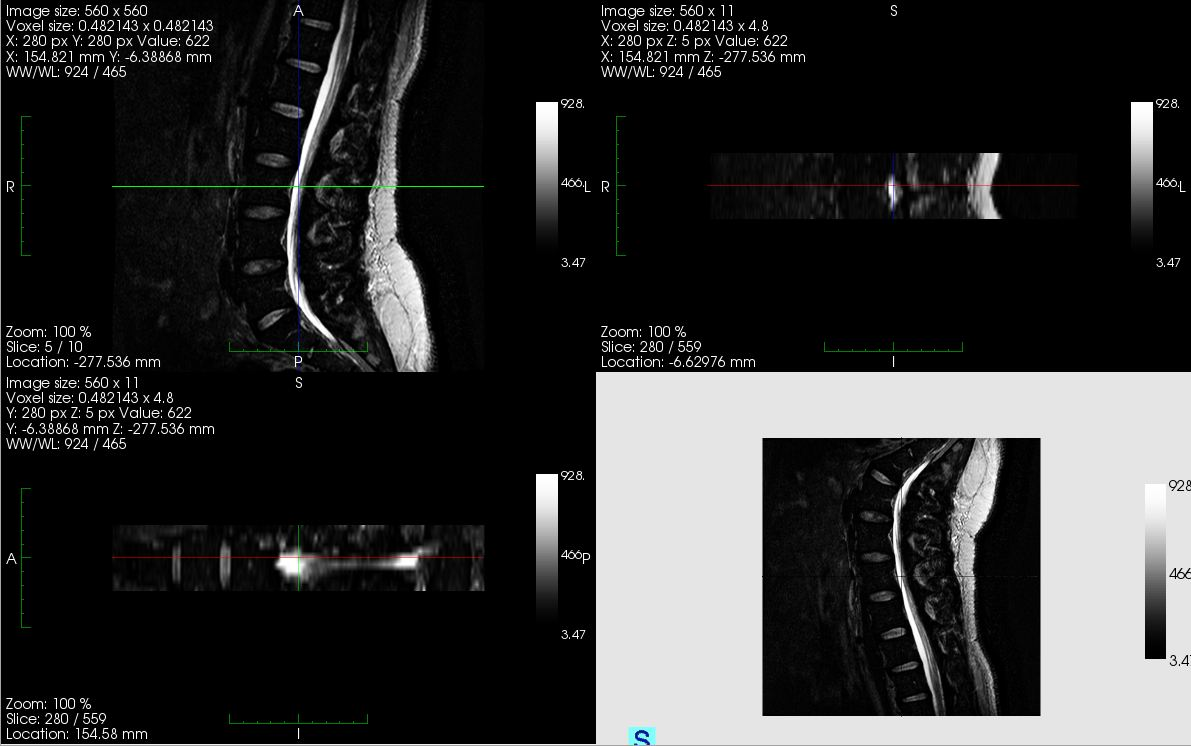
\includegraphics[width=0.9\textwidth,height=0.9\textwidth]{Text/IMG/MPR_Medinria.jpg}

\subsection{Objektový návrh Dicom-Presenteru}
Zadání bylo do stávajícího programu přidat podporu multiplanární rekonstrukce. Jelikož přidání MPR znamená zásah do stávajícího objektového návrhu programu, je nutné se nejprve stručně seznámit se stávajícím objektovým návrhem programu.

V programu DicomPresenter je vykreslování snímků na obrazovku realizováno kooperací několika různých tříd. V první řadě je možné vidět třídu, která zajišťuje zobrazení jednotlivých snímků, manipulaci se snímky uživatelem - tato třída se nazývá Workspace, neboli pracovní plocha. Program DicomPresenter umožňuje mít takovýchto pracovních ploch otevřeno hned několik a tak byly vytvořeny dvě další třídy. Jedna se stará o uložení pracovních tříd v paměti počítače - WorkspaceManager. Druhá třída je pak potřeba k přepínání mezi pracovnímí plochami uživatelem.

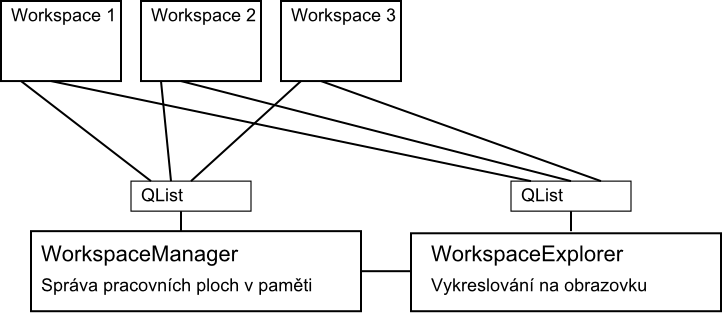
\includegraphics[width=0.9\textwidth]{Text/IMG/WorkspaceManager.png}

Do tohoto modelu je nutné někam zařadit novou třídu, která zajistí funkčnost multiplanární rekonstrukce. Byla tedy vytvořena nová třída podobná třídě Workspace, která nebude zobrazovat několik různých Dicom snímků, ale bude zobrazovat vždy jen jeden Dicom snímek v různých řezech. Bylo nutné zaručit, aby se uživatel mohl přepínat mezi novou pracovní plochou s multiplanární rekonstrukcí a mezi všemi starými pracovními plochami.

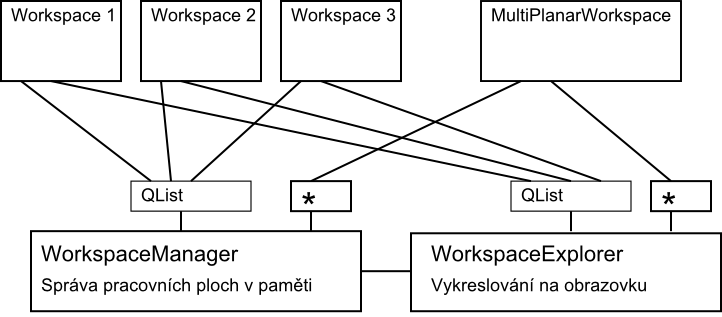
\includegraphics[width=0.9\textwidth]{Text/IMG/MultiPlanar.png}


\begin{comment}
Základním pojmen v objektovém návrhu DP je pracovní plocha (třída Workspace). Multiplanární rekonstrukce bude zobrazena na takové pracovní ploše. V této stati popíšeme třídy, jež úzce souvisí s pracovními plochami.

Pracovní plocha je reprezentována třídou Workspace. Třída Workspace se stará především o správu snímků s nimiž uživatel manipuluje a pak jejich vykreslení na obrazovku.

Třída WorkspaceManager se pak stará o uložení snímků v paměti programu. Třída vlastní objekt Qt knihovny QList, což je seznam, ve kterém jsou uloženy ukazatele na otevřené pracovní plochy.

Třída WorkspaceExplorer je pak třídou, která má na starosti grafické rozhraní, to znamená, že zajišťuje uživateli možnost manipulace s pracovními plochami: jejich otevírání, zavírání, přepínaní se mezi nimi.

Původní koncept, jak přidat do programu nový tip pracovní plochy, jež bude umožňovat multiplanární rekonstrukci byl takový, že rozdělíme třídu Workspace na dvě třídy. Více abstraktní funcke společné stávající pracovní ploše a nové pracovní ploše s MPR by pak mohly být odděleny v abstraktní třídě (nazvěme ji pro přehlednost MetaWorkspace). Tyto abstraktní funkce společné pro oba typy pracovních ploch jsou např.: vytváření animací, změna velikosti pracovní plochy, vykreslování obsahu pracovní plochy do frame bufferu atd.

Bohužel se ukázalo, že nový typ pracovní plochy bude od původní dosti odlišný ve funkčnosti, takže bylo vhodnější  vytvořit zcela odlišný typ pracovní plochy.

Pro multiplanární rekonstrukci tedy byl vytvořen nový typ pracovní plochy: třída PlanarWorkspace. Nová třída je v zásadě odlišná od původních pracovních ploch. Původní pracovní plochy obsahovali funkce pro přídávání jednotlivých snímků na obrazovku, pro přeskupování snímků atd. Všechny tyto funkce budou v pracovní ploše pro multiplanární rekonstrukci nepotřebné.

\end{comment}

\subsection{Implementace multiplanární rekonstrukce v třídě Image}
Multiplanární rekonstrukce je implementována tak, že v třídě Image byly vytvořeny nové funkce pro vykreslení tří na sebe kolmých řezů z trojrozměrné textury. Funkcím, jsou vždy předány souřadnice společného průsečíku tři dvourozměrných ploch, které zobrazujeme.

\begin{lstlisting}[label=DicomImageClass,caption={První část souboru \texttt{Window.cpp} se zdrojovým kódem třídy reprezentující okno programu.}]
void CGLImage::DrawToTextureSliceZ(TPlanarCrossPosition crossposition){
	glBindFramebufferEXT(GL_FRAMEBUFFER_EXT, iFBOZ);

 	glEnable(GL_TEXTURE_3D);
	glBindTexture( GL_TEXTURE_3D, iTexture->GetTextureID ());

	glEnable(GL_TEXTURE_2D);
	glBindTexture(GL_TEXTURE_2D, iSliceZ);

	glBegin(GL_QUADS);
	glColor4f( 1., 0., 0., 1.);
	glTexCoord3d(0,1,crossposition.z); 	glVertex2d(0,0);
	glTexCoord3d(1,1,crossposition.z); 	glVertex2d(1,0);
	glTexCoord3d(1,0,crossposition.z); 	glVertex2d(1,1);
	glTexCoord3d(0,0,crossposition.z);	glVertex2d(0,1);
	glEnd();

	glBindTexture(GL_TEXTURE_2D, 0);
	glDisable(GL_TEXTURE_2D);

	glBindTexture( GL_TEXTURE_3D, 0);
	glDisable(GL_TEXTURE_3D);

	glBindFramebufferEXT(GL_FRAMEBUFFER_EXT, 0);
}
\end{lstlisting}

Jak vidíme ve výpisu kódu, řez je pořizován z třírozměrné textury (řádky 12-15) a je kreslen do FrameBufferu (aktivace frame bufferu ř. 2), respektive pak do dvojrozměrné textury (aktivace textury ř. 7,8), která je uložena v paměti OpenGL. Z této textury je pak řez překreslen na obrazovku:

\begin{lstlisting}[label=DicomImageClass,caption={První část souboru \texttt{Window.cpp} se zdrojovým kódem třídy reprezentující okno programu.}]
void CGLImage::DrawSliceZ(){
	glEnable( GL_TEXTURE_2D );
	glBindTexture(GL_TEXTURE_2D, iSliceZ);
	glBegin( GL_QUADS );
	glTexCoord2d(0,0); 	glVertex2d(0,0.5);
	glTexCoord2d(1,0);		glVertex2d(0.5,0.5);
	glTexCoord2d(1,1);		glVertex2d(0.5,1);
	glTexCoord2d(0,1);		glVertex2d(0,1);
	glEnd();
	glBindTexture(GL_TEXTURE_2D, 0);
	glDisable(GL_TEXTURE_2D);
}
\end{lstlisting}

Změna v tom, z jaké části snímku bude pořizován aktuální řez je prováděna na základě uživatelských akcí, je tedy popsána a počítána ve funkcích Qt knihovny: mousePressEvent, mouseMoveEvent. Zajímavostí je, že PlanarWorkspace je objekt v hiearchii Qt podřazený objektu QWidget, který odpovídá hlavnímu oknu aplikace. Tedy všechny uživatelské akce zachycuje QWidget, který je pak předává podřazeným objektům.

V třídě PlanarWorkspace bylo tedy nutné definovat funkce mousePressEvent a mouseMoveEvent. Úkolem je toto: když uživatel klikne na jeden ze tří řezů, zapamatujme si pozici kurzoru. Když uživatel pohne myší v jednom ze směrů, tak podle toho přepočítejme pozici odpovídajícího řezu.

Ve funkci mousePressEvent tedy zjistíme na který z řezů uživatel klikl a zapamatujeme si pozici myši:

\begin{lstlisting}[label=DicomImageClass,caption={První část souboru \texttt{Window.cpp} se zdrojovým kódem třídy reprezentující okno programu.}]
void CGLPlanarWorkspace::mousePressEvent(QMouseEvent *event){
	int thisSizeX = this->GetSize().x();
	int thisSizeY = this->GetSize().y();
	int mousePositionX = event->x();
	int mousePositionY = event->y();
	if((mousePositionX<thisSizeX/2)&&(mousePositionY<thisSizeY/2)){
		UserManipulatingSlice = 'z';
		CGLWidget::GetInstance()->setCursor(QCursor(Qt::BlankCursor));
		iEventHistory->setX(mousePositionX);	
		iEventHistory->setY(mousePositionY);
		*iCursorHistory = QCursor::pos();
	}
	if((mousePositionX>thisSizeX/2)&&(mousePositionY<thisSizeY/2)){
 		...
	}
	if((mousePositionX<thisSizeX/2)&&(mousePositionY>thisSizeY/2)){
 		...	
	}
}
\end{lstlisting}

Na výpisu kódu je vidět, že si pozici dokonce zapisujeme dvakrát. To je zajímavý jev. Pozici kurzoru myši totiž lze počítat v absolutních hodnotách vzhledem k obrazovce počítače, nebo také v relativních hodnotách vzhledem k oknu aplikace. Pro výpočet do jakého ze tří oken s řezem textury uživatel klikl je výrazně přehlednější používat relativní souřadnice vzhledem k oknu aplikace (vyhneme se tak složitým přepočtům, když uživatel přemístí okno jinam, nebo dokonce na jiný monitor). Pokud ale chceme kurzor myši umístit po akci uživatele zpět na původní místo, což zde využíváme, je nutné tuto novou pozici zadávat v absolutních souřadnících vzhledem k obrazovce.

V těle funkce mouseMoveEvent pak počítáme o kolik uživatel pohl myší, myš vracíme na původní místo a dále nastavujeme nové souřadnice řezů. Dále je potřeba ošetřit situaci, kdy uživatel nastavuje souřadnice poblíž přípustné hranice. Na konci pak voláme překreslení OpenGL, aby se změny promítli na obrazovce.

\begin{lstlisting}[label=DicomImageClass,caption={První část souboru \texttt{Window.cpp} se zdrojovým kódem třídy reprezentující okno programu.}]
void CGLPlanarWorkspace::mouseMoveEvent(QMouseEvent *event){
	int mouseAfterMovePositionX = event->x();
	int mouseAfterMovePositionY = event->y();
	QCursor::setPos(*iCursorHistory);
	if(UserManipulatingSlice == 'z'){
		int dx = mouseAfterMovePositionX - iEventHistory->x();
		int dy = iEventHistory->y() - mouseAfterMovePositionY;
		if ((iPlanarCrossPosition.x+(float)dx/(float)iSensitivity>0.) && (iPlanarCrossPosition.x+(float)dx/(float)iSensitivity<1.))
			iPlanarCrossPosition.x=iPlanarCrossPosition.x+(float)dx/(float)iSensitivity;
		if ((iPlanarCrossPosition.y+(float)dy/(float)iSensitivity>0.) && (iPlanarCrossPosition.y+(float)dy/(float)iSensitivity<1.))
			iPlanarCrossPosition.y=iPlanarCrossPosition.y+(float)dy/(float)iSensitivity;
	}
	if(UserManipulatingSlice == 'x'){
 		...
	}
	if(UserManipulatingSlice == 'y'){
 		...
	}
	CGLWidget::GetInstance()->updateGL();
}
\end{lstlisting}




%%%%%%%%%%%%%%%%%%%%%%  DODATKY  %%%%%%%%%%%%%%%%%%%%%%

%\chapter{Dodatky}
%\section{Import kódu}
%\input{Text/07.Import.tex}

%%%%%%%%%%%%%%%%%%%%%%  LITERATURA  %%%%%%%%%%%%%%%%%%%%%%

\nocite{*}				% zobrazuj i necitovane primarni zdroje
\bibliography{Text/Literatura}
\nocitesec{*}				% sek. zdroje
\bibliographysec{Text/Zdroje}
\bibliographyurl{Text/Odkazy}


%%%%%%%%%%%%%%%%%%%%%%  PŘÍLOHY %%%%%%%%%%%%%%%%%%%%%%

% \chapter{Přílohy}

% \input{vnitrek_priloha1.tex} % pøíloha 1: vložená z externího souboru
% \input{vnitrek_priloha2.tex} % pøíloha 2: vložená z externího souboru



\end{document}

